%%%%%%%%%%%%%%%%%%%%%%%%%%%%%%%%%%%%%%%%%%%%%%%%%%%%%%%%%%%%%%%%%%%%%%%%
\raggedbottom
%                                                                      %
%     File: Thesis_Background.tex                                      %
%     Tex Master: Thesis.tex                                           %
%                                                                      %
%     Author: Andre C. Marta                                           %
%     Last modified :  4 Mar 2024                                      %
%                                                                      %
%%%%%%%%%%%%%%%%%%%%%%%%%%%%%%%%%%%%%%%%%%%%%%%%%%%%%%%%%%%%%%%%%%%%%%%%

\chapter{Theoretical background}
\label{chapter:Background}

This chapter covers the key concepts and theoretical background necessary to understand the work presented in this thesis. It begins by describing the \acrshort{maxcut} problem and discussing elements of computational complexity, reinforcing the rationale behind this research. The state-of-the-art algorithms for solving the \acrshort{maxcut} problem, both classical and hybrid quantum-classical, are then examined. After a brief introduction to quantum computing, the chapter explores hybrid quantum-classical computing and variational quantum algorithms in greater depth. Specifically, the Quantum Approximate Optimization Algorithm (\acrshort{qaoa}) and the Qubit-Efficient \acrshort{maxcut} Heuristic (\acrshort{qemc}) are analyzed, as they play a pivotal role in this study.

% Include state-of-the-art somewhere?! - Maybe in the "State-of-the-Art" section. I've tried to include this in the "The Maximum Cut Problem & Computational Complexity" section.

% Insert your chapter material here.

% Some overview of the underlying theory about the topic... - Here, I should describe mathematical preliminaries, quantum computing, variational quantum algorithms, and the \acrshort{maxcut} problem. I should also mention the importance of hybrid quantum-classical computing and the potential of combining QAOA and QEMC. Could also make sense to mention computational complexity.

% Remember to define an acronym the first time it is used.

% The full acronym can be \acrfull{mdo}, that includes both its long definition~\acrlong{mdo} and short definition~\acrshort{mdo}.


%%%%%%%%%%%%%%%%%%%%%%%%%%%%%%%%%%%%%%%%%%%%%%%%%%%%%%%%%%%%%%%%%%%%%%%%
\section{The Maximum Cut Problem \& Computational Complexity}
\label{section:MaxCut_Comp._Complexity}

The \acrshort{maxcut} problem, a fundamental problem in graph theory and combinatorial optimization, involves partitioning a graph \( G = (V, E) \) into two disjoint subsets, \( S_1 \) and \( S_2 \), such that the number of edges connecting vertices from different subsets is maximized. Formally, the objective is to find a partition \( (S_1, S_2) \) that maximizes:

\begin{equation}\label{eq:Cut}
\text{Cut}(S_1, S_2) = \sum_{(u, v) \in E} \chi(u, v),
\end{equation}
where \( \chi(u, v) = 1 \) if \( u \) and \( v \) belong to different subsets, and \( \chi(u, v) = 0 \) if they belong to the same subset. This quantity is referred to as the "cut" of the partition $(S_1, S_2)$. Pictorially, this can be represented as cutting the edges of the graph (Figure \ref{fig:MaxCut}), hence the name \acrshort{maxcut}. What we describe here is the un-directed, un-weighted \acrshort{maxcut} problem. A more general formulation would involve the specific graph's adjacency matrix, $W_{ij}$.

Since the \acrshort{maxcut} problem is NP-hard, finding an optimal solution efficiently is a significant computational challenge, especially as the graph size grows. However, researchers have developed various approximation algorithms and heuristics to approach near-optimal solutions in a reasonable time, including both classical and quantum approaches (cf. subsections \ref{section:Classical-State-of-the-Art} and \ref{section:Hybrid-Quantum-Classical-State-of-the-Art}). These methods are designed to tackle the intrinsic complexity of the problem, providing practical solutions that have real-world applications. As mentioned earlier, the \acrshort{maxcut} problem finds use in a variety of fields, including machine learning \cite{937505}, statistical physics \cite{Barahona_Grötschel_Jünger_Reinelt_1988}, circuit design \cite{Barahona_Grötschel_Jünger_Reinelt_1988}, and data clustering \cite{10.1007/11893318_21}.

\begin{figure}[H]
  \centering
  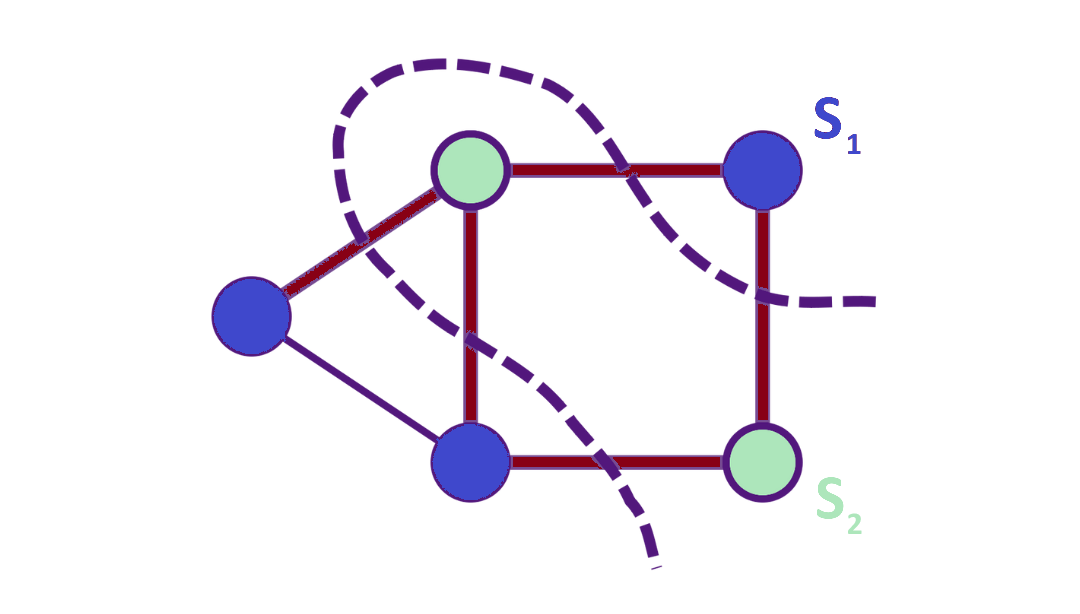
\includegraphics[width=\textwidth]{Figures/Diagrams/MaxCut.png}
  \caption{An example of a graph with a partition that maximizes the number of cut edges (red). Note that the \acrshort{maxcut} partition might not be unique.}
  \label{fig:MaxCut}
\end{figure}

% Discussion on Computational Complexity
We previously mentioned that the \acrshort{maxcut} problem is well-known to be NP-hard. (Indeed, it [decision version] even appears on Karp's original list of NP-complete problems, from 1972 \cite{Karp2010}.) Let's explore what this means in more detail. The computational complexity class of a problem is defined by the computational resources required to solve it, such as time or memory. Although there are many complexity classes (see the \href{https://complexityzoo.net/Complexity_Zoo}{Complexity Zoo}), the following four are key to our discussion:

\begin{enumerate}
  \item \textbf{P (Polynomial time)}: Problems that can be solved in polynomial time by a deterministic Turing machine, indicating they are computationally efficient.
  \item \textbf{NP (Non-deterministic Polynomial time)}: Problems that can be verified in polynomial time if given a solution, but finding the solution may not be as straightforward. Therefore, if you guess a solution, you can confirm its correctness quickly.
  \item \textbf{NP-hard (Non-deterministic Polynomial time hard)}: Problems that are at least as challenging as the most difficult problems in NP. If you could solve an NP-hard problem in polynomial time, you would be able to solve all problems in NP efficiently.
  \item \textbf{NP-complete (Non-deterministic Polynomial time complete)}: Problems that belong to NP but are also NP-hard. If you can solve one NP-complete problem efficiently, all problems in NP would become efficiently solvable.
\end{enumerate}

The \acrshort{maxcut} problem in its \textbf{optimization form} – "Given a graph $G$, find the maximum cut" – is NP-hard. This implies that if you could find an efficient solution to \acrshort{maxcut}, you could also solve all other NP problems reliably. That would include, e.g., the boolean SATisfiability problem (\acrshort{sat}), knapsack problem, decision version of the traveling salesman problem, clique problem, and more \cite{NP-problems}. This potential for broad application drives interest in developing high-performance algorithms for \acrshort{maxcut}. Alternatively, the \acrshort{maxcut} problem can be formulated as a \textbf{decision problem} – "Given a graph $G$ and an integer $k$, determine if there is a cut of size at least $k$ in $G$." This formulation is NP-complete. NP-complete status indicates that a problem is both in NP, allowing polynomial-time verification, and at least as hard as any other problem in NP, making it central to computational theory and offering crucial insights into the boundary between efficiently solvable and intractable problems. Although our focus is on the NP-hard version of the problem, it's important to understand the significance of the NP-complete formulation.

% The \acrshort{maxcut} problem, in particular, has a wide range of applications, such as in machine learning \cite{937505}, statistical physics \cite{Barahona_Grötschel_Jünger_Reinelt_1988}, circuit design \cite{Barahona_Grötschel_Jünger_Reinelt_1988}, and data clustering \cite{10.1007/11893318_21}.

% Describe the \acrshort{maxcut} problem, that we intend to solve, in an approximate manner. - Explain its importance and potential applications. Also, briefly mention computational complexity and the NP-hardness of the problem.

% \acrshort{maxcut} is actually NP-Hard, not NP-Complete. (Actually, depends on how you phrase it. For it to be NP-Complete, it'd have to be the decision version of the problem: "Is this the \acrshort{maxcut} partition?: Yes/No." I think so, but re-check this.)

% NP-Complete = NP and NP-Hard. (Instead of NP + NP-Hard.) Notation! I think I should write it like this.

%%%%%%%%%%%%%%%%%%%%%%%%%%%%%%%%%%%%%%%%%%%%%%%%%%%%%%%%%%%%%%%%%%%%%%%%
\subsection{Classical State-of-the-Art Algorithms for MaxCut}
\label{section:Classical-State-of-the-Art}

% I need to define, e.g., the concept of approximation ratio (AR). And, put it in the Glossary too!

Over the years, a variety of algorithms have been proposed to solve the \acrshort{maxcut} problem, ranging from exact solutions to various approximations, including heuristics and other techniques. In this work, we focus on scaling these algorithms to handle bigger graphs, which is why exact algorithms are not discussed – they quickly become impractical for large instances. Instead, our attention is on approximation algorithms, which are more suitable for larger scales\footnote{In this section, "larger/bigger graphs" will often refer to graphs with many hundreds to a few thousand nodes.}.

Approximation algorithms aim to find solutions that are close to optimal, often with a guaranteed Approximation Ratio (\acrshort{ar}). This is a measure of the performance of an approximation algorithm, representing the worst-case deviation between the algorithm's solution and the optimal solution. Formally, this can be expressed as: (For the Goemans-Williamson (\acrshort{gw}) Algorithm \cite{GW-Algorithm}, e.g.)\footnote{The actual value is $\alpha=\operatorname*{min}_{0\,\leq\,\theta\leq\pi}\,\frac{2}{\pi}\,\frac{\theta}{1\,-\,\cos\,\theta} > \,0.878$.}$$r_A^{GW} = \frac{\text{Cut}_{\text{GW}}}{\text{MaxCut}} \approx 0.87856,$$
where $\text{Cut}_{\text{GW}}$ is the worst-case "cut" value obtained by the Goemans-Williamson Algorithm, and $\text{MaxCut}$ is the \acrshort{maxcut} value. The \acrshort{ar} is a crucial metric for evaluating the quality of an approximation algorithm, providing insight into its effectiveness. The closer the \acrshort{ar} is to $1$, the better the algorithm's performance. In literature, this worst-case approximation ratio might also be referred to as the \textit{performance guarantee} $\rho$, often appearing alongside designations such as $\rho$-approximation algorithm. Using this nomenclature, the Goemans-Williamson Algorithm is a $0.87856$-approximation algorithm for \acrshort{maxcut} (i.e., $\rho = 0.87856$).

Building on this, two commonly used \textbf{approximation algorithms} are:

\begin{itemize}
  \item \textbf{Goemans-Williamson Algorithm} \cite{GW-Algorithm}: This popular approximation algorithm achieves a performance guarantee of approximately $0.87856$, leveraging Semidefinite Programming (\acrshort{sdp}) and a randomized rounding technique. (This will be further developed below, in subsubsection \nameref{subsubsection:GW_Algorithm}.)
  \item \textbf{Spectral Methods} \cite{Spectral-MaxCut}: These techniques employ eigenvalues and eigenvectors of the adjacency matrix to identify effective cuts. While spectral methods may offer quicker computational speeds compared to other approximation strategies (e.g. \acrshort{gw}), they may not consistently provide the optimal approximation ratios. Performance-wise, the leading spectral algorithm, Trevisan's algorithm, using Soto's refined analysis \cite{Soto-MaxCut}, features a worst-case approximation ratio of $0.614$.
\end{itemize}

\textbf{Heuristic} and \textbf{metaheuristic algorithms} offer another approach, focusing on finding solutions more quickly, albeit without guaranteed approximation ratios. They are typically employed when computational efficiency is prioritized over achieving the best possible approximation ratio. These algorithms include:
\begin{itemize}
  \item \textbf{Greedy Algorithms} (Described in \cite{Spectral-MaxCut}): These build solutions incrementally, following a greedy approach. Mathematically, we start with $S_1, S_2 = \emptyset$. In each step of the algorithm, we choose a vertex $v \in V$ yet to be assigned to $S_1$ or $S_2$. Then, we add $v$ to $S_1$ or $S_2$ by choosing the larger of the two cuts $(S_1 \cup \{v\}, S_2)$ and $(S_1, S_2 \cup \{v\})$ at this step. Repeat until all vertices are assigned to a set.
  \item \textbf{Simulated Annealing} \cite{SA_MaxCut}: Employs a probabilistic optimization approach, inspired by metallurgical annealing, to iteratively explore the solution space, gradually reducing the acceptance of worse solutions ("temperature") over time to converge towards near-optimal solutions.
  \item \textbf{Genetic Algorithms} \cite{GA_MaxCut}: These algorithms, rooted in evolutionary principles, employ selection, crossover, and mutation techniques to iteratively generate solutions for the \acrshort{maxcut} problem, evolving from an initial population of diverse partitions towards improved solutions.
\end{itemize}
Reiterating, these approximation and heuristic methods offer scalable solutions for the \acrshort{maxcut} problem, making them more suitable for larger graphs where exact methods are not feasible.

Of all the mentioned approaches, we will now elaborate on the Goemans-Williamson algorithm, which currently stands as the most effective approximation method for \acrshort{maxcut}, boasting the best-known performance guarantee to date ($0.87856$). Its detailed explanation is particularly relevant as we plan to utilize it in benchmarking our proposed algorithms later on. We opt for \acrshort{gw} over other options for one obvious reason: Our aim is to push the boundaries of \acrshort{maxcut} algorithms, thus it is logical to compare against the top-performing method. (We do not use any of the heuristic/metaheuristic algorithms, as they do not provide performance guarantees, and we are interested in having a benchmark to compare against.)

\subsubsection{Goemans-Williamson Algorithm}
\label{subsubsection:GW_Algorithm}

In this subsubsection, we shall present the Goemans-Williamson Algorithm in greater detail. This approximation algorithm, developed by Michel X. Goemans and David P. Williamson in 1995 \cite{GW-Algorithm}, is a cornerstone in the field of combinatorial optimization, particularly for the \acrshort{maxcut} problem. The algorithm leverages semidefinite programming to construct a solution that is then rounded to provide a near-optimal cut. Semidefinite programming involves optimizing a linear function of a symmetric matrix while adhering to linear equality constraints and the requirement that the matrix be positive semidefinite. This programming paradigm finds utility across diverse fields such as control theory, nonlinear programming, geometry, and combinatorial optimization, showcasing its versatility and applicability. (These applications are detailed in \cite{GW-Algorithm} and references therein.)

Formally, the Goemans-Williamson Algorithm can be described as follows. (We will use the original formulation, from \cite{GW-Algorithm}, presenting a distilled version of the most important aspects of their description.) Given a graph, with vertex set $V = \{1,..., n\}$ and non-negative weights $w_{ij} = w_{ji}$ for each pair of vertices $i$ and $j$, the weight of the maximum cut $w(S_1, S_2)$ is given by the following integer quadratic program\footnote{Note that we use the general formulation here, contemplating the possibility of weighted graphs, i.e., we do not restrict ourselves to un-weighted graphs.}:

\vspace{-5mm}
\begin{equation}\label{eq:Graph_Cut}
  \begin{split}
  &\mathrm{Maximize}\;\;\frac{1}{2}\sum_{\stackrel{i < j:}{(i,j)\in E}}w_{i j}(1-y_{i}y_{j}) \\
  (Q)\qquad\qquad\qquad&\operatorname{Subject\;to:}y_{i}\in\{-1,1\}\qquad\qquad\forall i\in V.
  \end{split}
\end{equation}

\sloppy
\noindent It is clear that the sets $S_1 = \{i|y_i=1\}$ and $S_2 = \{i|y_i=-1\}$ correspond to a cut of weight $w(S_1, S_2) = \frac{1}{2}\sum_{\stackrel{i < j:}{(i,j)\in E}}w_{ij}\left(1-y_{i}y_{j}\right)$. This  represents the same quantity as the aforementioned $\text{Cut}(S_1, S_2) = \sum_{(u, v) \in E} \chi(u, v)$ (Eq. \ref{eq:Cut}), in the un-weighted case. Explicitly, in words, the sum in Eq. \ref{eq:Graph_Cut} is to be taken over all the graph's edges $(i, j)$, with $y_{i}$ representing node-$i$'s associated set: $y_{i}=+1$, if node-$i$ $\in S_1$, or $y_{i}=-1$, when node-$i$ $\in S_2, \forall i \in V$.

Given that solving this integer quadratic program is NP-hard \cite{GW-Algorithm}, we explore relaxations of $(Q)$. These are obtained by relaxing some of the constraints of $(Q)$, and extending the objective function to the larger space. Consequently, all solutions of $(Q)$ are feasible for the relaxation, and the optimal value of the relaxation serves as an upper bound for $(Q)$'s optimal value. We interpret $(Q)$ as constraining $y_i$ to be a $1$-dimensional unit vector. A number of possible relaxations involve allowing $y_i$ to be a multidimensional vector $v_i$ of unit Euclidean norm. As the linear space spanned by the vectors $v_i$ has dimension at most $n$ (number of graph nodes), we can assume that these vectors belong to $\mathbb{R}^{n}$. More precisely, they belong to the $n$-dimensional unit sphere, $S_n$. At this point, so as to make sure that the resulting optimization problem is, indeed, a relaxation, we must define the cost function such that it reduces to $\frac{1}{2}\sum_{i<j}w_{i j}(1-y_{i}y_{j})$ for vectors lying in a $1$-dimensional space. One way to do this is to replace $y_{i}y_{j}$ with the inner product $v_{i} \cdot v_{j}$ in the expression for $w(S_1, S_2)$. The resulting relaxation, $(P)$, reads:

\vspace{-5mm}
\begin{equation}
  \begin{split}
  &\mathrm{Maximize}\;\;\frac{1}{2}\sum_{\stackrel{i < j:}{(i,j)\in E}}w_{i j}(1-v_{i} \cdot v_{j}) \\
  (P)\qquad\qquad\qquad&\operatorname{Subject\;to:}v_{i}\in S_n \qquad\qquad\forall i\in V.
  \end{split}
\end{equation}
In the context of this semidefinite programming relaxation, the \acrshort{gw} algorithm follows these steps:
\begin{enumerate}
  \item Solve $(P)$, thus obtaining an optimal set of vectors $v_{i}$;\vspace{-2.5mm}
  \item Let $r$ be a vector uniformly distributed on the unit sphere, $S_n$;\vspace{-2.5mm}
  \item Set $S_1 = \{i|v_{i} \cdot r \geq 0\}$ and $S_2 = \{i|v_{i} \cdot r < 0\}$.
\end{enumerate}
In other words, we choose a random hyperplane through the origin (with $r$ as its normal), in $n$ dimensions, and partition the vertices according to whether the vectors $v_{i}$ lie "above" ($v_{i} \cdot r \geq 0$) or "below" ($v_{i} \cdot r < 0$) this hyperplane. Those above the hyperplane are assigned to $S_1$, and those below to $S_2$.

Furthermore, it can be shown that the \acrshort{gw} algorithm has a performance guarantee of:
\begin{equation}
  \alpha=\operatorname*{min}_{0\,\leq\,\theta\leq\pi}\,\frac{2}{\pi}\,\frac{\theta}{1\,-\,\cos\,\theta} > \,0.878.
\end{equation}
A detailed proof elucidating the appearance of this $0.878$ value is present in section $3$ of \cite{GW-Algorithm}.

Computationally, one defines the positive semidefinite matrix $X \in \mathbb{R}^{n \times n}$, with $X_{ii} = 1$ and $X_{ij} = v_{i} \cdot v_{j} = v_{i}^{T} v_j$, $\forall i, j \in V$. Then, we can solve the following semidefinite program:
\begin{equation}
  \begin{split}
  &\mathrm{Maximize}\;\;\frac{1}{2}\sum_{\stackrel{i < j:}{(i,j)\in E}}w_{i j}(1-X_{ij}) \\
  (N)\qquad\qquad\qquad&\operatorname{Subject\;to:}X_{ii} = 1, \forall i\in V, X \succeq 0.
  \end{split}
\end{equation}
We do possess effective tools and techniques for solving semidefinite programs (e.g., interior point methods), enabling the efficient determination of a highly satisfactory $X$ matrix. From there, we can extract the vectors $v_{i}$, by performing the square root operation on the matrix $X$. The resulting matrix's columns, or rows – $X$ is symmetric – will correspond to the desired vectors $v_{i}$. This outlines the process for solving $(P)$ as listed earlier.

% Re-read all of this and potentially re-write some things. I'm also not sure if I should just cite the GW paper, for defining semidefinite programming.

% Describe the state-of-the-art algorithms for the \acrshort{maxcut} problem. - Mention classical algorithms, such as the Goemans-Williamson algorithm, and quantum algorithms, such as the Quantum Approximate Optimization Algorithm (QAOA) and the Qubit-Efficient \acrshort{maxcut} Heuristic (QEMC) algorithm.

%%%%%%%%%%%%%%%%%%%%%%%%%%%%%%%%%%%%%%%%%%%%%%%%%%%%%%%%%%%%%%%%%%%%%%%%

\subsection{Hybrid Quantum-Classical State-of-the-Art Algorithms for MaxCut}
\label{section:Hybrid-Quantum-Classical-State-of-the-Art}

A number of different hybrid quantum-classical algorithms have been proposed to solve the \acrshort{maxcut} problem, leveraging the unique properties of quantum computing to potentially outperform purely classical algorithms. They are designed to exploit quantum superposition and entanglement to explore the solution space more efficiently. In this section, we will briefly mention the state-of-the-art hybrid quantum-classical algorithms for \acrshort{maxcut}, focusing on the Quantum Approximate Optimization Algorithm (\acrshort{qaoa}) and the Qubit-Efficient \acrshort{maxcut} Heuristic Algorithm (\acrshort{qemc}). Due to their variational nature, these algorithms do not have a theoretical performance guarantee, but they have shown promising results in practice.

Presently, the Quantum Approximate Optimization Algorithm (\acrshort{qaoa}), initially introduced in \cite{farhi2014quantum}, is one of the top candidates for achieving meaningful quantum advantage with near-term quantum devices. Although, \acrshort{maxcut}-wise, it has a substantial limitation: it requires a number of qubits equal to the number of graph nodes. This is a significant drawback, as it severely limits the algorithm's scalability to bigger graphs. Hence, why it is believed that \textit{"QAOA for Max-Cut requires hundreds of qubits for quantum speed-up"} \cite{Guerreschi2019}. After all, our classical algorithms work just fine for small graphs, which is why we do not present performance metrics for basic \acrshort{qaoa}. Alternatively, different \acrshort{qaoa} variations have been proposed to address the issue of high qubit requirements, such as QAOA-in-QAOA \cite{zhou2022qaoainqaoa}, which partitions a large graph into many smaller subgraphs, each of which is easily solved using a separate \acrshort{qaoa} instance. Afterwards, these results are joined together by working through another, this time \textbf{weighted}, \acrshort{maxcut} problem. This approach in particular has proven to yield competitive or even better performance over the best known classical algorithms, i.e. \acrshort{gw}, for graphs up to $2000$ nodes.

A separate problem one might face when implementing \acrshort{qaoa}, that also hinders its application to larger graphs, has to do with qubit connectivity\footnote{Qubit connectivity refers to the pattern or arrangement of connections between qubits in a quantum computing system, determining which qubits can interact directly with each other.}, as \acrshort{qaoa} might require specific connectivity patterns that are not natively available in present-day \acrshort{nisq} devices. To implement these, we are often required to utilize a number of $2$-qubit SWAP gates, which degrade the algorithm's performance by introducing extra noise in the system, and hence errors in our results. Therefore, a parallel line of work has been to develop \acrshort{qaoa} variations that have lesser connectivity requirements, in the sense that they do not depend on arbitrary qubit connectivity. For example, Parity-QAOA \cite{ender2022modular,Ender2023parityquantum} was designed for quantum chips with planar lattice geometry (Figure \ref{fig:Planar_lattice_geometry}), requiring only nearest-neighbour connectivity. Although it necessitates more qubits, it entirely solves this problem.

\begin{figure}[H]
  \centering
  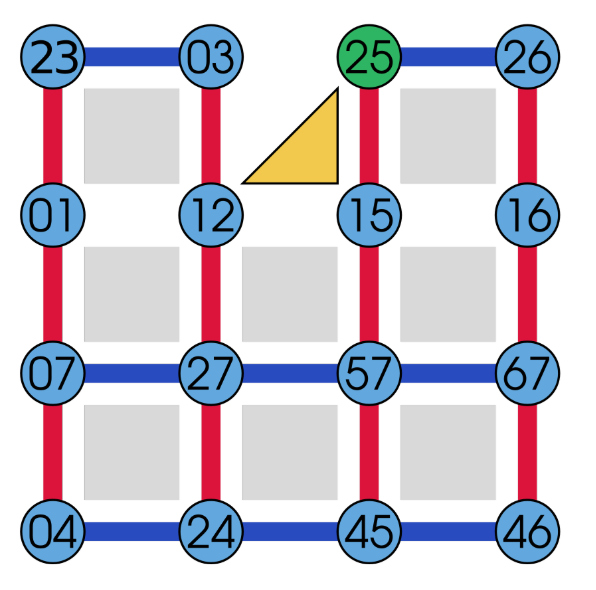
\includegraphics[width=0.5\textwidth]{Figures/Diagrams/Planar_lattice_geometry.png}
  \caption{Planar lattice geometry illustration: the circular nodes represent the physical qubits, each of which can interact directly with its nearest neighbours. The lines represent terms of the driver Hamiltonian, from Parity-QAOA \cite{ender2022modular}. The numbers refer to edges in the original graph. Image reproduced from \cite{ender2022modular}.}
  \label{fig:Planar_lattice_geometry}
\end{figure}

Furthermore, the Qubit-Efficient \acrshort{maxcut} Heuristic Algorithm (\acrshort{qemc}), introduced in \cite{tenecohen2023variational}, is a quantum-classical hybrid algorithm that aims to solve the \acrshort{maxcut} problem using fewer qubits than \acrshort{qaoa}, therefore extending its applicability to larger graphs. It has shown cutting-edge performance in practice, occasionally surpassing the classical state-of-the-art, i.e. \acrshort{gw}, for graphs up to $2048$ nodes. The novelty of this algorithm is that it opens up the door for quantum devices to be used for large \acrshort{maxcut} instances, previously unfeaseble due to qubit number limitations, which rendered \acrshort{qaoa} computations for such large graphs impossible. As was already mentioned, \acrshort{qemc} allows for an exponential compression in the number of needed qubits, enabling its utilization on today's quantum hardware for considerably larger graphs than what would be possible with traditional \acrshort{qaoa}. However, this exponential compression also makes it efficiently simulable classically, which effectively defeats its purpose as a quantum algorithm. For this reason, \acrshort{qemc} is termed a quantum-inspired classical algorithm and, by definition, will not produce any quantum advantage. Either way, we include it in this subsection, since it can always be implemented as a \acrshort{vqa} on current-day \acrshort{nisq} devices.

More recently, different algorithms have been proposed in an attempt to reduce the number of qubits required for larger graphs, without falling into the trap of efficient classical simulability. (After all, we are looking for quantum advantage.) Polynomial compression-based algorithms, such as that proposed in \cite{sciorilli2024largescale}, have too shown promising results. This one in specific \cite{sciorilli2024largescale} is, to the best of our knowledge, boasting the highest quality attained experimentally on sizes up to $7000$ graph nodes, competitive with state-of-the-art classical solvers. Not only that, but their specific qubit-efficient encoding brings in a super-polynomial mitigation of barren plateaus\footnote{In \acrshort{vqa} analysis, barren plateaus are characterized by a vanishing expectation value of \(\nabla{\mathcal{L}}\) over random parameter initializations and an exponential decay (in the number of qubits, \(n\)) of its variance, where \(\mathcal{L}\) refers to the loss function. These are flat regions of the parameter space, impeding optimization.} as a built-in feature, which constitutes a significant advantage over other \acrshort{vqa}\textcolor{gray}{s}. Curiously enough, our initial idea for the \acrshort{iqaqe} Framework is quite similar to what is explored in \cite{sciorilli2024largescale}. However, we believe our concept to be somewhat more general, by not assuming \textit{a priori} a polynomial compression in the number of qubits.

% I believe this part is okay, now. Maybe re-read it one more time, and ask Carolina to do the same. Add the Parity-QAOA figure, illustrating planar lattice geometry?

% Find papers showing that QAOA has been used/employed for solving \acrshort{maxcut} in x graphs.

% Describe, albeit briefly, the state-of-the-art quantum algorithms for the \acrshort{maxcut} problem. - Mention the Quantum Approximate Optimization Algorithm (QAOA) and the Qubit-Efficient \acrshort{maxcut} Heuristic (QEMC) algorithm. No need to explain them, as they will be further developed in the next sections.

%%%%%%%%%%%%%%%%%%%%%%%%%%%%%%%%%%%%%%%%%%%%%%%%%%%%%%%%%%%%%%%%%%%%%%%%
\section{Quantum Computing Primer}
\label{section:QC_Primer}

In this section, we present a brief introduction to quantum computing, focusing on its fundamental ideas and principles. We begin with an overview of the general concepts, followed by a discussion of quantum gates and circuits, crucial for understanding quantum algorithms. This groundwork will prepare us to delve into the specifics of variational quantum algorithms and their application to the \acrshort{maxcut} problem.

% I feel like I should add some more mathematics to this. Refer to Bence's master thesis as a reference, e.g. Done!

% Remember to go over the papers in the 'papers' folder! Add those that aren't there yet! Maybe re-check whether to include some of the 'misc' references (IonQ/Google qubit-types, e.g. Isn't there a paper where this is refered?) I should try to replace these with actual papers. The Pennylane tutorials are fine though, I think. They even provide their references, which can be cross-checked any time. For the Google, i.e., can utilize the Sycamore paper, for quantum advantage. There's probably something similar for IonQ, and others (maybe not quantum advantage, but still). Update: this is done!

% Change all the important people's names to italics? I've removed italics from everyone's names now. Done!

% Remember that we have an 80 page maximum limit! This can be extended to 100 in appendices, and the like.

\subsection*{General concepts and mathematical formalism}
\vspace*{-5mm}{\scriptsize \noindent (This description is inspired by \cite{nielsen2010quantum}.)}

Quantum computing makes use of the foundational principles of quantum mechanics in an attempt to extract some sort of quantum advantage from them. Instead of using classical binary digits, quantum computers use their quantum analog, qubits. In practice, qubits can be any two-state quantum system. Said states are, unequivocally, associated with the states $\ket{0}$ and $\ket{1}$, conventionally, very much like in classical computing when one uses bits. The primary distinction lies in the fact that a qubit, being a quantum system, can exist in a superposition of both states generally denoted as: (We use Dirac notation.)
\begin{equation}
  \mathcal{H}^2 \ni \ket{\psi} = \alpha \ket{0} + \beta \ket{1},
\end{equation}
where $\alpha, \beta \in \mathbb{C}$, with $\abs{\alpha}^2 + \abs{\beta}^2 = 1$. This ensures probability normalization to $1$, as, according to the famous Born rule, the probability of measuring the qubit in state $\ket{0}$ is $\abs{\bra{0}\ket{\psi}}^2 = \abs{\alpha}^2$, and in state $\ket{1}$ is $\abs{\bra{1}\ket{\psi}}^2 = \abs{\beta}^2$.

In the same vein, one can compose (represented by the tensor product) $n$ qubits to obtain an $n$-qubit state:
\begin{equation}\label{eq:n_qubit_state}
  \ket{\psi}=\bigotimes_{i=0}^{n-1}(\alpha_{i}\ket{0}_{i}\ +\beta_{i}\ket{1}_{i}).
\end{equation}
More generally, we can express an arbitrary pure state of $n$ qubits, $\ket{\psi}$, by a normalized linear combination of the computational basis states $\ket{b_0 b_1 ... b_{n-1} b_n} \coloneq \ket{b_0} \otimes \ket{b_1} \otimes ... \otimes \ket{b_{n-1}} \otimes \ket{b_n}$:
\begin{equation}\label{eq:general_n_qubit_state}
  \ket{\psi} = \sum_{\boldsymbol{b} \in \{0, 1\}^{n}} \alpha_{\boldsymbol{b}} \ket{b_0 b_1 ... b_{n-1} b_n},
\end{equation}
where $\sum_{\boldsymbol{b} \in \{0, 1\}^{n}} \abs{\alpha_{\boldsymbol{b}}}^2 = 1$. This superposition phenomenon (mathematically characterized by the linear combination of basis states), utterly impossible in classical physics, brings unprecedented computational power under certain scenarios, as it introduces a kind of built-in parallelism in quantum computing, a highly desirable feature for any computational scheme.

In addition to this, quantum computing also exploits entanglement as a resource. Entanglement allows for intricate correlations between qubits, which have no classical counterpart, and are believed to offer computational speed-ups, although it is yet unclear exactly how. An entangled state, by definition, is one that cannot be expressed as the tensor product of individual qubit states, i.e., it cannot be represented in the form of Eq. \ref{eq:n_qubit_state}. The most famous example of entangled states are the Bell states, representing what are known as two-qubit (or bipartite) maximally entangled states. Such Bell states are reproduced below:
\begin{equation} % Check if these are correct!
  \begin{aligned}
  \ket{\Phi^+} &= \frac{1}{\sqrt{2}}(\ket{00} + \ket{11}), \quad
  \ket{\Phi^-} = \frac{1}{\sqrt{2}}(\ket{00} - \ket{11}), \\
  \ket{\Psi^+} &= \frac{1}{\sqrt{2}}(\ket{01} + \ket{10}), \quad
  \ket{\Psi^-} = \frac{1}{\sqrt{2}}(\ket{01} - \ket{10}).
  \end{aligned}
\end{equation}
Indeed, these states cannot be expressed as a tensor product of two individual qubit states. From a practical standpoint, Bell states frequently serve as foundational elements in advanced techniques like quantum teleportation and quantum cryptography. Quantum Key Distribution (\acrshort{qkd}) protocols, for example, frequently rely on entangled Bell pairs to distribute secure keys for encrypting and decrypting messages.

Another key topic in quantum information theory is the distinction between pure and mixed states. So far, we have only been treating pure states, which are represented by a single ket vector in some Hilbert space. Mixed states, on the other hand, are represented by density matrices, which are positive semidefinite matrices with unit trace. These matrices are used to describe a statistical ensemble of pure states. The density matrix $\rho$ of a pure quantum state $\ket{\psi}$ is defined as:
\begin{equation}
  \rho = \dyad{\psi}{\psi}.
\end{equation}
In the more general case of a statistical ensemble of pure states $\ket{\psi_i}$, each with probability $p_i$, the density matrix $\rho$ is given by:
\begin{equation}
  \rho = \sum_i p_i \dyad{\psi_i}{\psi_i}.
\end{equation}
It's crucial to avoid confusing this with superposition, as a mixed state comprises a statistical ensemble of pure states, while superposition pertains to a single state that is a linear combination of other states. For instance, the state $\ket{\psi_S} = \frac{1}{\sqrt{2}}\left(\ket{0} + \ket{1}\right)$ represents a superposition of $\ket{0}$ and $\ket{1}$, whereas the state $\rho_M = \frac{1}{2}\left(\dyad{0}{0} + \dyad{1}{1}\right)$ denotes a mixed state, signifying that half the states in the ensemble are in state $\ket{0}$ and the other half in state $\ket{1}$. Unlike the probabilistic mixture ($\rho_M$), the superposition ($\ket{\psi_S}$) can exhibit quantum interference, hence why it is important to distinguish between the two. If desired, this distinction can also be observed in the off-diagonal terms of the density matrix, referred to as coherences, which are responsible for quantum interference effects: the off-diagonal terms of $\rho_{M}$ are zero, whereas those of $\rho_{S} = \dyad{\psi_S}{\psi_S} = \frac{1}{4}\left(\dyad{0}{0} + \dyad{0}{1} + \dyad{1}{0} + \dyad{1}{1}\right)$ are not.

\vspace*{-2.5mm}
\subsubsection*{Types of qubits – physical implementations}
\vspace*{-2.5mm}
Currently, numerous quantum computing architectures are in competition and the ultimate victor remains uncertain. Nevertheless, the most prominent architectures have qubits composed of either photons \cite{slussarenko2019photonic, Xanadu_Photonics}, neutral atoms (using Rydberg states) \cite{Henriet2020quantumcomputing, Wu_2021}, trapped ions \cite{bruzewicz2019trapped}, semiconductors \cite{Chatterjee2021}, or, most notably, superconducting circuits \cite{Huang_2020, SC_Qubits} – employed by giants like IBM and Google in their quantum processors. Looping back to the definition of a qubit, considering a photonic quantum computer, it becomes rather straightforward and natural to map the photon's vertical and horizontal polarizations to the $\ket{0}$ and $\ket{1}$ states, respectively\footnote{Note that there are alternative ways (other than polarization) to encode quantum information in photons for quantum computing.}. Once again, this mapping is analogous to how classical computing maps the current/no current states to $1$ and $0$.

The next step is to understand how these so-called quantum circuits act on our qubits, and how they can be used to perform quantum computations. This is where quantum gates come into play.

% Things that are yet to be done in regards to this section:
% Mention the Hadamard gate somewhere! It's a fundamental gate in quantum computing. Done!

% Present proof? Using only R_x and R_z, I know this is possible. Done!

% Wikipedia link? Find something else, maybe? Probably. Done!

\vspace*{-2.5mm}
\subsection*{Quantum gates and circuits}
\vspace*{-2.5mm}
Presently, quantum computers are being designed predominantly with a circuit-based architecture. These circuits serve as the quantum equivalent of classical logic circuits, however, instead of the typical AND, OR, and NOT gates, quantum circuits feature quantum gates. These gates apply specific transformations to qubits, based on their definitions, taking an initial state $\ket{\psi}$ to an output state $\ket{\phi} = U\ket{\psi}$, for some gate $U$, \textbf{designed to be unitary}, i.e., $U^{\dagger}U = UU^{\dagger} = I$, where $I$ is the identity matrix. Unitary transformations preserve the normalization of quantum states and the inner product between states, which are essential properties in quantum mechanics. Additionally, they ensure that quantum operations are reversible, meaning that information is not lost during computation. This [unitary gates] can also be seen as a natural consequence of the Schrödinger equation, governing the time evolution of quantum systems, requiring said evolution to be described by a unitary operator.

The most frequently used quantum gates consist of rotations around each of the three Cartesian axes, represented as complex exponentials of the Pauli $x$, $y$ and $z$ matrices ($\sigma_x$, $\sigma_y$ and $\sigma_z$). The Pauli matrices are defined as: (Note the alternative notation, $\boldsymbol{X}$, $\boldsymbol{Y}$ and $\boldsymbol{Z}$.)
\begin{equation}
  \boldsymbol{X} \coloneq \sigma_x =
  \begin{pmatrix}
    0 & 1 \\
    1 & 0
  \end{pmatrix},
  \quad
  \boldsymbol{Y} \coloneq \sigma_y =
  \begin{pmatrix}
    0 & -i \\
    i & 0
  \end{pmatrix},
  \quad
  \boldsymbol{Z} \coloneq \sigma_z =
  \begin{pmatrix}
    1 & 0 \\
    0 & -1
  \end{pmatrix}.
\end{equation}
Furthermore, when we mention rotations, these are to be seen in the Bloch sphere, which is a geometrical representation of the pure state space of a two-level quantum system, an illustration of which can be seen in Figure \ref{fig:Bloch_sphere}.

\begin{figure}[H]
    \centering
    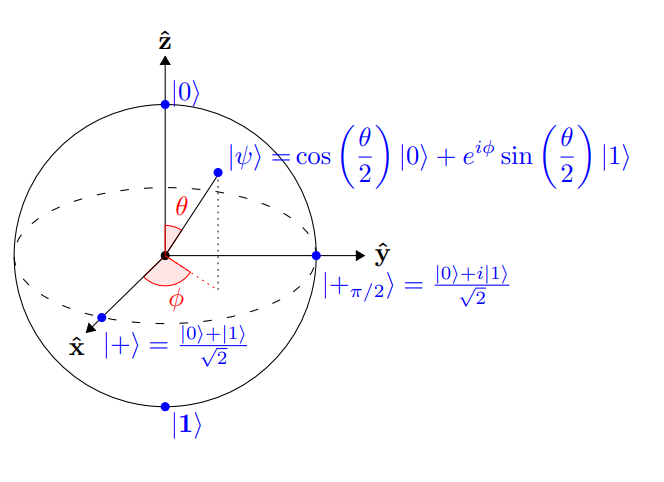
\includegraphics[width=0.75\textwidth]{Figures/Diagrams/Bloch_sphere.png}
    \caption{Bloch sphere representation. The sphere's north  and south poles correspond to states $\ket{0}$ and $\ket{1}$, respectively. Reproduced from \cite{Bloch_Sphere_Ref}.}
    \label{fig:Bloch_sphere}
\end{figure}
\noindent The aforementioned rotation gates can be written as: $R_x(\theta) = e^{-i\theta\boldsymbol{X}/2}$, $R_y(\theta) = e^{-i\theta\boldsymbol{Y}/2}$, and $R_z(\theta) = e^{-i\theta\boldsymbol{Z}/2}$. In matrix form, this reads:
\begin{equation}
  \resizebox{0.90\hsize}{!}
  {$
  % X rotation matrix
  R_x(\theta) =
  \begin{pmatrix}
    \cos\left(\frac{\theta}{2}\right) & -i\sin\left(\frac{\theta}{2}\right) \\
    -i\sin\left(\frac{\theta}{2}\right) & \cos\left(\frac{\theta}{2}\right)
  \end{pmatrix},
  \quad
  % Y rotation matrix
  R_y(\theta) =
  \begin{pmatrix}
    \cos\left(\frac{\theta}{2}\right) & -\sin\left(\frac{\theta}{2}\right) \\
    \sin\left(\frac{\theta}{2}\right) & \cos\left(\frac{\theta}{2}\right)
  \end{pmatrix},
  \quad
  % Z rotation matrix
  R_z(\theta) =
  \begin{pmatrix}
    e^{-i\frac{\theta}{2}} & 0 \\
    0 & e^{i\frac{\theta}{2}}
  \end{pmatrix},
  $}
\end{equation}
These will frequently appear in quantum circuits, as they are the most basic quantum gates, in the sense that all other single-qubit gates can be re-constructed from them, i.e., for any unitary single-qubit gate $U$, one can always find a decomposition $U=e^{i\phi}R_{Z}(\gamma)R_{X}(\beta)R_{Z}(\alpha)$ (formally proven in \cite{Barenco_1995}).
% Present proof? Using only R_x and R_z, I know this is possible. I should present a reference for this, though. Done!

For illustrative purposes, to elucidate how single-qubit gates act on qubits, it is quite simple to verify that the $\sigma_x$ matrix (alternative symbol, $\boldsymbol{X}$) behaves exactly like a NOT gate. This correspondence is established through a $180^{\circ}$ rotation around the $x-$axis. Mathematically,
% X|0> = |1> 
\begin{equation}
\boldsymbol{X} = 
\begin{pmatrix}
0 & 1 \\
1 & 0
\end{pmatrix},
\end{equation}
such that:
\begin{equation}
\boldsymbol{X}\ket{0}
=
\begin{pmatrix}
0 & 1 \\
1 & 0
\end{pmatrix}
\begin{pmatrix}
1 \\
0
\end{pmatrix}
=
\begin{pmatrix}
0 \\
1
\end{pmatrix}
=
\ket{1}.
\end{equation}
Another essential gate found in most quantum algorithms is the Hadamard gate. It can be represented as the following linear combination of $\boldsymbol{X}$ and $\boldsymbol{Z}$ matrices: $H = \frac{1}{\sqrt{2}}\left(\boldsymbol{X} + \boldsymbol{Z}\right)$, and is particularly useful for creating superpositions, as it maps the state $\ket{0}$ to $\frac{1}{\sqrt{2}}(\ket{0} + \ket{1}) \coloneq \ket{+}$, and $\ket{1}$ to $\frac{1}{\sqrt{2}}(\ket{0} - \ket{1}) \coloneq \ket{-}$.
% Re-read this bit on the Hadamard gate.

In addition to these simple one-qubit quantum gates, there are also gates designed for multiple qubits. For instance, consider the controlled-NOT gate (CNOT), which does exactly what its name suggests: if the control qubit is in state $\ket{1}$, it applies NOT to the test qubit, whereas if it is in state $\ket{0}$ instead, nothing happens. The CNOT gate is also quite prevalent in quantum circuits, playing a vital role in creating entanglement between qubits, which is a crucial resource in quantum computing. The circuit representation and equivalent matrix form of the CNOT gate are presented below, in Figure \ref{fig:CNOT}.

\begin{figure}[htbp]
  \centering
  \begin{subfigure}[t]{0.45\textwidth}
      \centering
      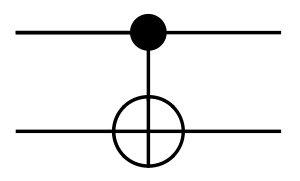
\includegraphics[width=.75\textwidth]{Figures/Diagrams/CNOT_Gate.png}
      \caption{CNOT gate – circuit representation. The black (filled) circle identifies the control qubit. The other qubit is the test qubit.}
      \label{fig:CNOT_Gate}
  \end{subfigure}
  \hfill
  \begin{subfigure}[t]{0.45\textwidth}
      \centering
      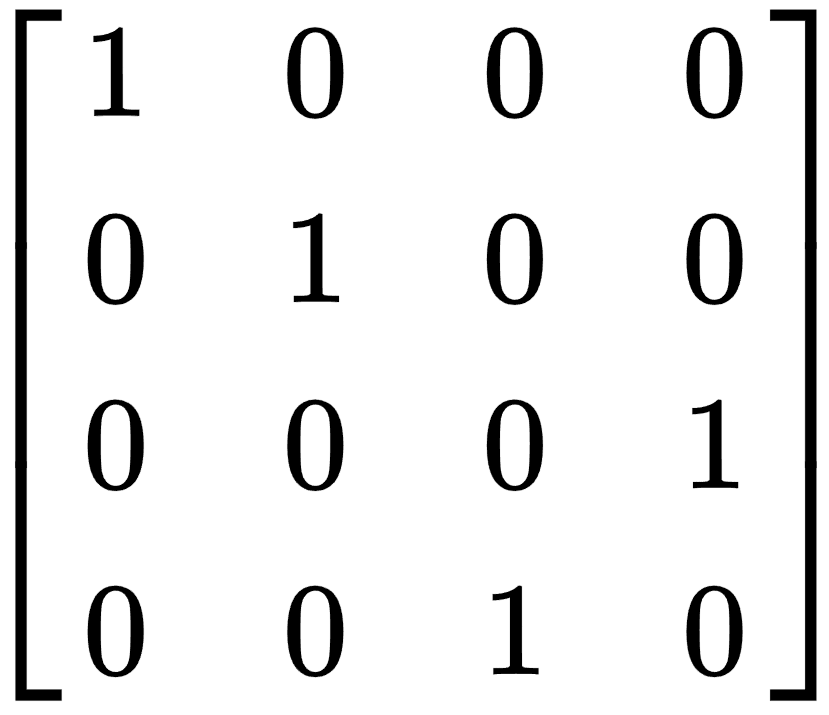
\includegraphics[width=.50\textwidth]{Figures/Diagrams/CNOT_Matrix.png}
      \caption{CNOT gate – equivalent matrix form.}
      \label{fig:CNOT_Matrix}
  \end{subfigure}
  \caption{Two-qubit gate example – the controlled-NOT gate.}
  \label{fig:CNOT}
\end{figure}

More generally, within a quantum circuit, an intricate network of interconnected qubits and gates collaborates to execute a specific algorithm. For example, the circuit depicted in Figure \ref{fig:QCircuit}, below, is designed for the implementation of the renowned Grover's search algorithm \cite{Grover}.

% Taken from Wikipedia. Should, then, include everything in my references!
\begin{figure}[H]
    \centering
    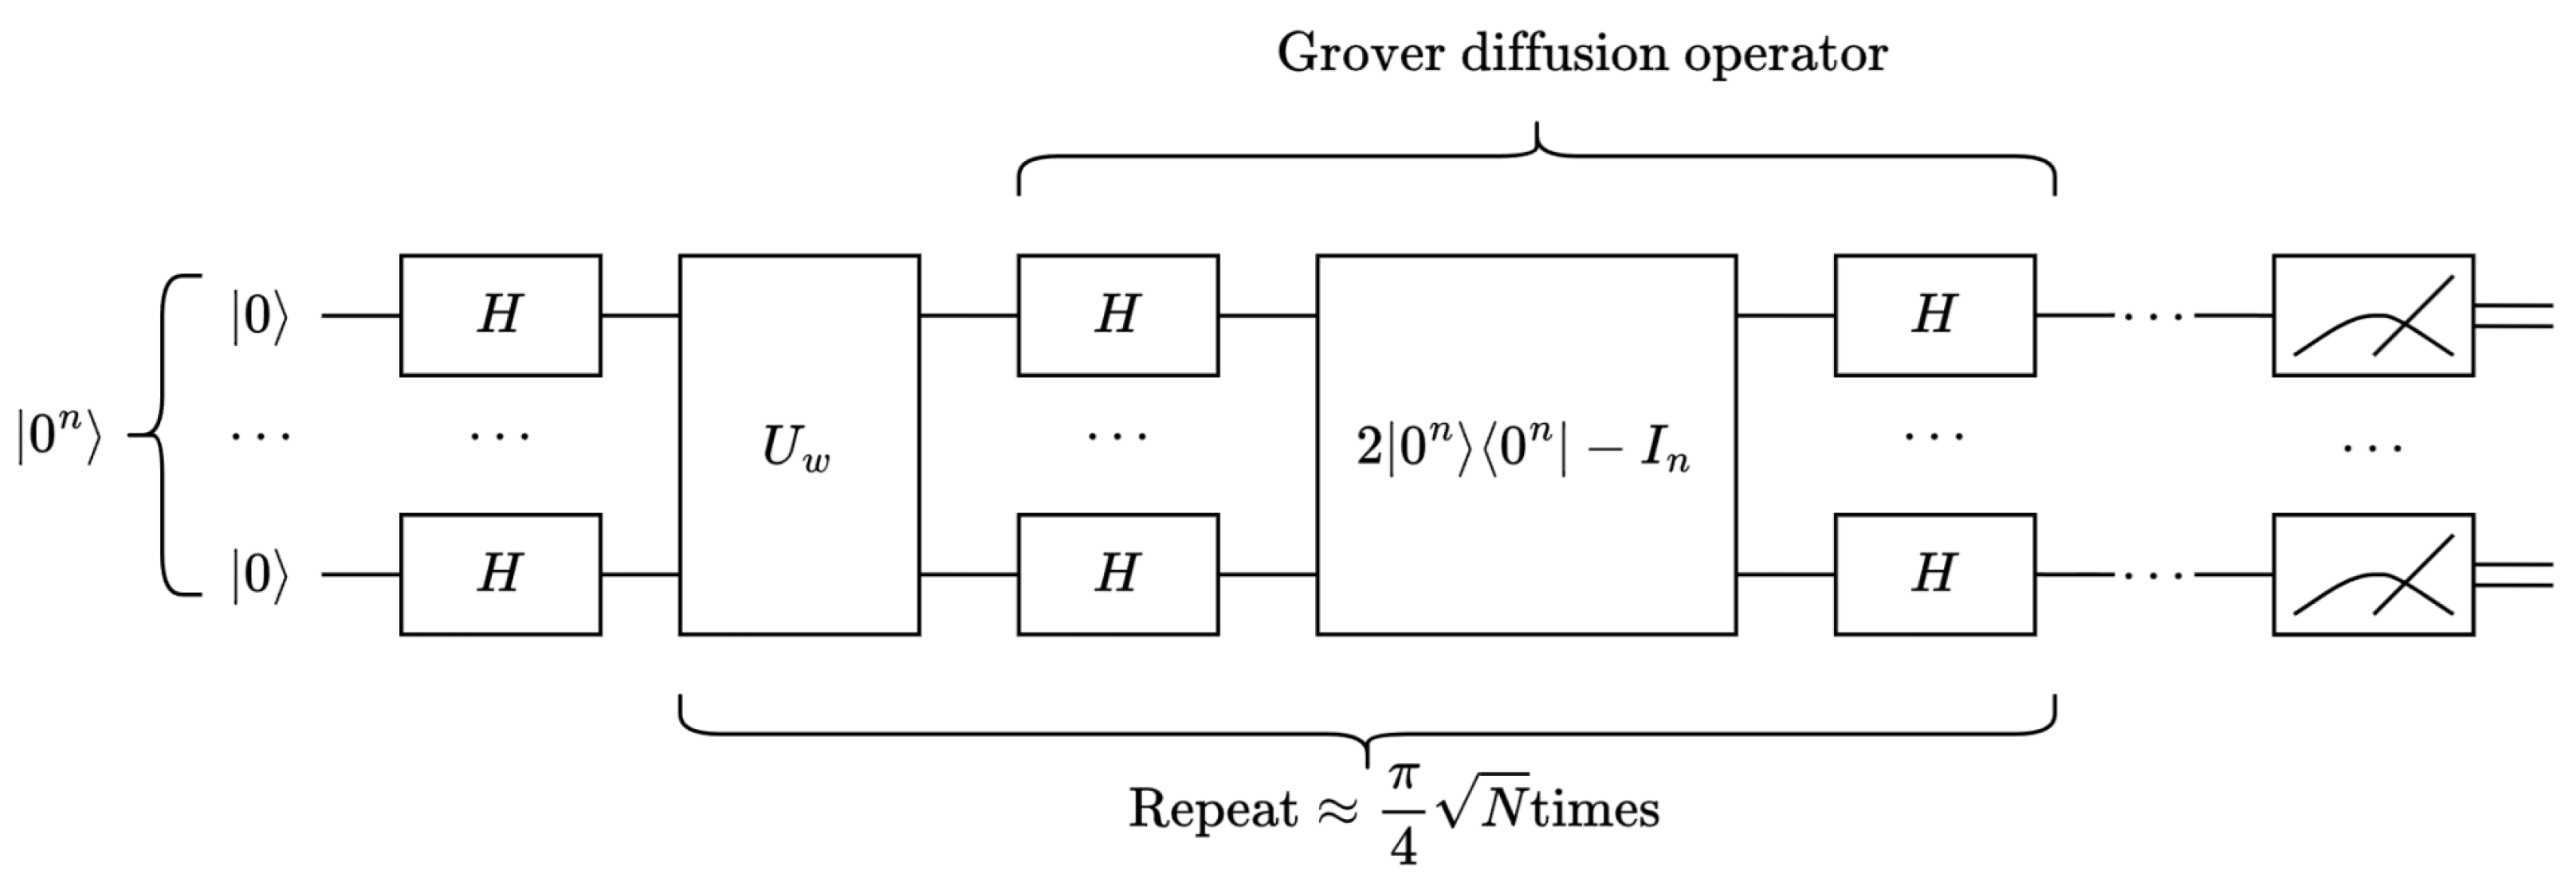
\includegraphics[width=\textwidth]{Figures/Diagrams/Grover_Circuit.png}
    \caption{Quantum circuit utilized in the famous Grover's search algorithm \cite{Grover}. Integraly reproduced from \cite{e26030216}.}
    \label{fig:QCircuit}
\end{figure}
\noindent This is a purely quantum algorithm, different from what we intend to explore in this work. Nevertheless, it serves as a good example of how quantum circuits can be used to implement complex quantum algorithms.

An additional point of interest is the potential for classical simulation of quantum circuits. Quantum gates, being akin to mathematical operators, can always be expressed in matrix form. Consequently, analyzing the impact of a series of quantum gates, i.e., a quantum circuit, on a specific quantum state is achievable by sequentially applying the relevant operators, as they appear in the circuit. At the end of this process, we arrive at a quantum state typically distinct from the initial state. This entire simulation can be executed classically. However, its scalability is severely limited, as the number of states, constituting our computational basis, representable with $n$ qubits grows exponentially, at a rate of $2^n$. As one might anticipate, this very quickly becomes unmanageable. Eventually, either memory constraints impede the storage of such extensive states, or the computations require so much time that the endeavor loses practicality. Effectively, simulating quantum computers becomes challenging beyond a few dozen qubits. Some tabletop calculations suggest that simulating $28$ qubits would necessitate approximately $13$ GB of memory, reaching the theoretical maximum capacity of a modern standard $16$ GB personal computer. It's important to note that for each additional qubit, memory requirements double. For instance, simulating $50$ qubits would demand about $54$ Petabytes of memory, and for $51$ qubits, approximately $108$ PB, and so forth. These estimations are based on the assumption that a complex number is stored as two Python floats, each requiring $24$ bytes of memory, thus a complex amplitude requires $48$ bytes of memory to be stored. Then, one such amplitude is required for each of the $2^{n}$ basis states, for $n$ qubits.

% This could be "Quantum Computing".

% The research should be supported with a comprehensive list of references.
% These should appear whenever necessary, in the limit, from the first to the last chapter.

% Regarding the exponential scaling: maybe it'd be interesting to provide some numbers. In other words, try to find the "greatest" number of qubits one can classically simulate, at the moment, and connect this to a number of bytes (memory-wise): Some Exabytes?

% I feel like if I am going to be including some text from my PIC2 report, I should further explain some of these things better.

% A reference can be cited in any of the following ways:
% %
% \begin{itemize}
%   \item Citation mode \#1 - \quad \cite{Marta:AeroBest2021}
%   \item Citation mode \#2 - \quad \citet{Marta:AeroBest2021}
%   \item Citation mode \#3 - \quad \citep{Marta:AeroBest2021}
%   \item Citation mode \#4 - \quad \citet*{Marta:AeroBest2021}
%   \item Citation mode \#5 - \quad \citep*{Marta:AeroBest2021}
%   \item Citation mode \#6 - \quad \citealt{Marta:AeroBest2021}
%   \item Citation mode \#7 - \quad \citealp{Marta:AeroBest2021}
%   \item Citation mode \#8 - \quad \citeauthor{Marta:AeroBest2021}
%   \item Citation mode \#9 - \quad \citeyear{Marta:AeroBest2021}
%   \item Citation mode \#10 - \quad \citeyearpar{Marta:AeroBest2021}
% \end{itemize}

% The references may include books~\cite{Marta:AeroBest2021}, articles in journals~\cite{Morgado:2022:SAMO}, part of a collection of books~\cite{jameson:adjointns}, articles in conferences~\cite{Alves:ICUAS:2022}, master theses~\cite{Pacheco:MSc} and PhD theses~\cite{Rodrigues:PhD}.

% Several citations can be made simultaneously as \cite{Campos:2021:QJMAM,Alexandre:2020:PLOS}.

% This is often the default bibliography style adopted (numbers following the citation order), according to the options:

% {\tt \textbackslash usepackage\{natbib\}} in file {\tt Thesis\_Preamble.tex},\\
% {\tt \textbackslash bibliographystyle\{abbrvnat\}} in file {\tt Thesis.tex}.\\

% Notice however that this style can be changed from numerical citation order to authors' last name with the options:

% {\tt \textbackslash usepackage[numbers]\{natbib\}} in file {\tt Thesis\_Preamble.tex},\\
% {\tt \textbackslash bibliographystyle\{abbrvunsrtnat\}} in file {\tt Thesis.tex}. \\

% Multiple citations are compressed when using the {\tt sort\&compress} option when loading the {\tt natbib} package as {\tt \textbackslash usepackage[numbers,sort\&compress]\{natbib\}} in file {\tt Thesis\_Preamble.tex}, resulting in citations like \cite{Pacheco:2024:JAUTO,Portugal:2024:MODELLING,Matos:2022:AEROSPACE,Rodrigues:2020:SAMO,Rodrigues:2019:RENE,Campos:2018:JSV,Rodrigues:2018:CAF,Campos:2015:GAFD,Marta:2014:JPP,Rodrigues:2014:SMO,Campos:2014:IJMS,Marta:2013:AIAAJ,Marta:2013:CAF,Marta:2010:CAF,Marta:2007:IJCFD}.


%%%%%%%%%%%%%%%%%%%%%%%%%%%%%%%%%%%%%%%%%%%%%%%%%%%%%%%%%%%%%%%%%%%%%%%%
\section{Hybrid Quantum-Classical Computing}
\label{section:HQCC}

% Other models. - Variational quantum algorithms, Parameterized quantum circuits, etc.

Hybrid quantum-classical computing refers to a computational approach that combines elements of both classical and quantum computing paradigms to leverage the strengths of each. In this model, classical processors and quantum processors work in tandem to solve complex problems more efficiently than either could achieve alone. This collaborative strategy aims to harness quantum computing's unique capabilities while mitigating the challenges and limitations associated with quantum systems, such as error correction and decoherence. As of today, the synergy between classical and quantum elements holds promise for addressing complex real-world problems in areas like optimization, machine learning, and cryptography (cf. Figure \ref{fig:VQAs_Applications}).

\subsection{Variational Quantum Algorithms}
\label{subsection:VQA}

% I've only just copied things from my PIC2 report. I still need to re-read everything and add more information, if I so deem important. Even this copy-paste'ing isn't done yet. Put this in a private GitHub repo., I think. [Good, for security reasons, in case somethings happens, I have a backup.] Done!

% In describing ansätze, I should mention that, in general, it is always better to use problem-inspired ansätze. If they're well designed/implemented, they should always yield better results. Also, when presenting examples of ansätze, I can show some images of those. Done!

% I should fact check some of what I say in the PIC2 report regarding problem-agnostic and -inspired ansätze. I feel like I might have said something wrong there. [About parameter number and depth, mostly, and, thus trainability.]

The hallmark of \acrshort{hqcc} is what are called variational quantum algorithms (\acrshort{vqa}\textcolor{gray}{s}), which correspond to hybrid quantum-classical algorithms, typically realized through a parameterized quantum circuit (\acrshort{pqc}). Additionally, as part of their implementation, the parameters are subjected to training in order to achieve the desired outcomes, by minimizing the value of a cost function. As such, \acrshort{vqa}\textcolor{gray}{s} can be thought of as the quantum analogue of highly successful machine-learning methods, such as neural networks. Moreover, since they outsource the circuit parameters' optimization to a classical optimizer, exterior to the quantum processor, \acrshort{vqa}\textcolor{gray}{s} leverage the full toolbox of classical optimization. As a whole, this approach has the added advantage of keeping the quantum circuit depth shallow, which, ultimately, helps in supressing the overall noise level. This is crucial, since it allows for these algorithms to be implemented in the current \acrshort{nisq} (Noisy Intermediate Scale Quantum) era, not requiring complete fault-tolerance to produce reasonable results. A wide array of possible applications has been examined for \acrshort{vqa}\textcolor{gray}{s}, essentially covering all the use cases envisioned by researchers for quantum computers (cf. Figure \ref{fig:VQAs_Applications}). Despite all this, it is important to note that \acrshort{vqa}\textcolor{gray}{s} are not without fault. There is still a lot of work to be done regarding their trainability, accuracy and efficiency. Either way, they are undoubtedly the most promising candidates for achieving useful quantum advantage in the near future, which is exactly why they have come under the spotlight, drawing the attention of numerous scientists over the past few years.

\begin{figure}[H]
  \centering
  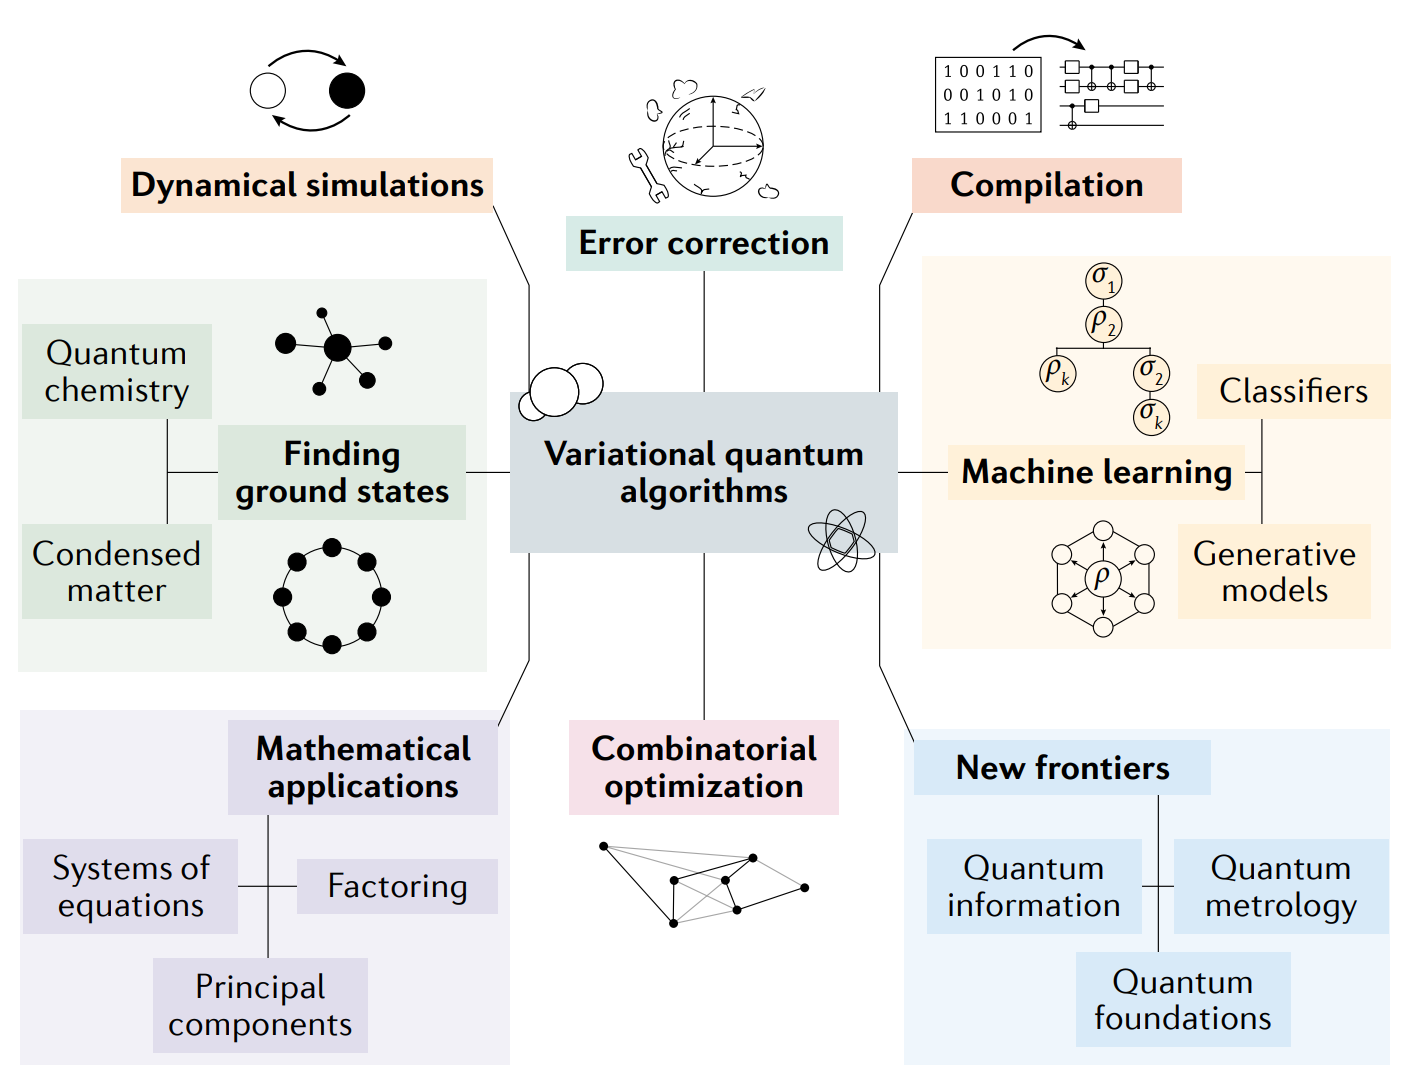
\includegraphics[width=0.65\textwidth]{Figures/Diagrams/VQAs_Applications.png}
  \caption{Applications of variational quantum algorithms. Sourced from \cite{Cerezo_2021} in its entirety.}
  \label{fig:VQAs_Applications}
\end{figure}

\begin{figure}[H]
  \centering
  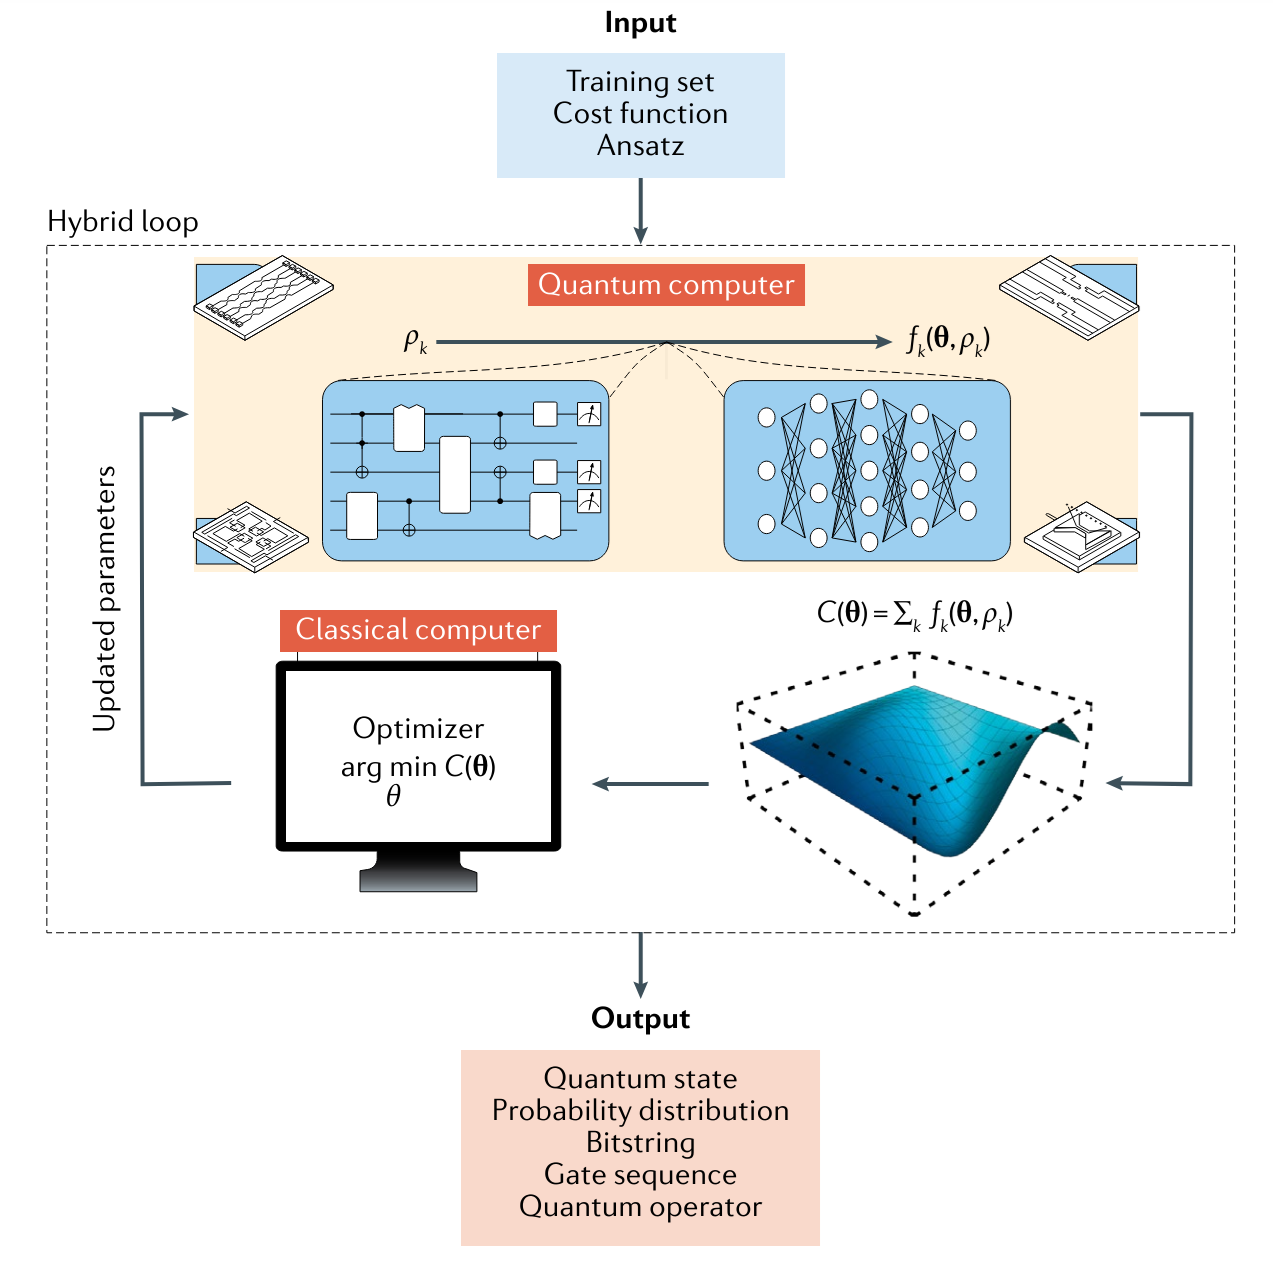
\includegraphics[width=0.65\textwidth]{Figures/Diagrams/VQA_Schematic.png}
  \caption{Schematic diagram of a variational quantum algorithm. Reproduced from \cite{Cerezo_2021}.}
  \label{fig:VQA_Schematic}
\end{figure}

% I should re-read EVERYTHING to see if there aren't many repetitions from previously mentioned things.

\subsubsection{Basic structure of a VQA}
\vspace*{-5mm}{\scriptsize \noindent (This description is heavily inspired by \cite{Cerezo_2021} and mirrors their section layout.)}

This section provides an overview of the essential components of \acrshort{vqa}\textcolor{gray}{s}. Kicking off the development of a \acrshort{vqa} involves defining a cost (or loss) function, $C$, that encodes the solution to the problem. Following this, an ansatz is suggested, that is a quantum circuit that relies on a set of continuous or discrete parameters, $\boldsymbol{\theta}$, subject to optimization. In other words, we propose the functional form/structure of the parameterized quantum circuit. Afterwards, the suggested ansatz undergoes training, within a hybrid quantum-classical loop (cf. Figure \ref{fig:VQA_Schematic}), to address the following optimization task
\begin{equation}\label{eq:Optimization}
  \boldsymbol{\theta}^{\star} = \arg \min_{\boldsymbol{\theta}} C(\boldsymbol{\theta}),
\end{equation}
corresponding to the minimization of the selected cost function. The distinctive feature of \acrshort{vqa}\textcolor{gray}{s} is their application of a quantum computer to estimate the cost function, $C(\boldsymbol{\theta})$, and its gradient, while relying on classical routines for the optimization of the parameters' values, $\boldsymbol{\theta}$. Next, we provide supplementary information for each step of the \acrshort{vqa} framework.

% Kind of a subsubsubsection.
\subsubsection*{\small Cost function}
An essential aspect of \acrshort{vqa}\textcolor{gray}{s} involves encoding the problem into an adequate cost function. Similar to classical machine learning, this function associates values of the trainable parameters, $\boldsymbol{\theta}$, with real numbers. At a more abstract level, the cost function defines a hypersurface, often termed the cost landscape (cf. Figure \ref{fig:VQA_Schematic}), in a way such that the optimizer's task is to then navigate across this landscape and discover its global minimum, as this would correspond to the sought-after solution. In many instances, it is beneficial and feasible to express the cost in the form:
\begin{equation}\label{eq:Cost}
    C(\boldsymbol{\theta}) = \sum_k f_k\left( Tr\left[O_k U(\boldsymbol{\theta}) \rho_k U^{\dagger}(\boldsymbol{\theta})\right] \right),
\end{equation}
for some set of functions $\{f_k\}$, where $U(\boldsymbol{\theta})$ is a parameterized unitary, $\boldsymbol{\theta}$ is composed of discrete and/or continuous parameters, $\rho_k$ are input states from a training set and $O_k$ are a set of observables. Note how the argument of $f_k$, $Tr\left[O_k U(\boldsymbol{\theta}) \rho_k U^{\dagger}(\boldsymbol{\theta})\right]$, corresponds to the expectation value of observable $O_k$, in state $\rho_k' = U(\boldsymbol{\theta}) \rho_k U^{\dagger}(\boldsymbol{\theta})$. Oftentimes, it is convenient to design the cost function to be given by the expectation value of a Hamiltonian (e.g., the cost Hamiltonian in \acrshort{qaoa}), which is why we mention that it is beneficial for it to have this specific form. Then, the minimization of the cost corresponds, unambiguously, to the determination of the ground-state energy. Additionally, one frequently uses Pauli operators, whose expectation values are rather easy to compute in practice.

Furthermore, when designing a cost function, we want it to be as faithful as possible, in the sense that its minimum should closely correspond to the desired solution. Likewise, it is imperative that we can efficiently estimate $C(\boldsymbol{\theta})$, as this is integral to the functionality of this method. So far, we have been taking this for granted. However, one must guarantee that this is indeed verified experimentally, otherwise we are not able to proceed.

% Kind of a subsubsubsection.
\subsubsection*{\small Ansätze}
Another crucial element of a \acrshort{vqa} is the ansatz. In broad terms, the ansatz's structure determines the nature of the parameters $\boldsymbol{\theta}$ and, consequently, how they can be optimized to minimize the cost. The design of an ansatz often relies on the specific requirements of the task, allowing for the creation of problem-inspired ansätze. However, certain ansatz architectures are generic and problem-agnostic, making them applicable even in scenarios where relevant information is lacking. As one might expect, problem-agnostic ansätze, being more general, will also, usually, require a greater number of parameters, which unsurprisingly hinders the optimization task. However, this also grants them more flexibility. On the other hand, problem-oriented ansätze are capable of assimilating problem-specific information into the structure of quantum circuits. This custom-fit approach can result in a reduction of the parameter space, making optimization more efficient, and lead to solutions that are more meaningful and interpretable. Furthermore, adopting such an approach might (at times, not always!) enable the use of shallower quantum circuits, thereby aiding in the reduction of overall noise levels. (Greater circuit depths require more quantum gates, which results in more noise.) When it all comes down to it, one should weigh the trade-off between accuracy and generality, and carefully assess resource utilization in the choice of ansatz. (Yet, for achieving optimal results tailored to a specific problem, it's always recommended to utilize problem-inspired ansätze. The challenge lies in their design. While it's tempting to opt for a problem-agnostic ansatz and consider the task done, problem-inspired designs consistently yield superior performance.) For illustration purposes, here are a few examples of commonly considered ansatz types: hardware-efficient ansätze (aimed at reducing circuit depth), unitary coupled clustered ansätze (for quantum chemistry simulations), quantum alternating operator ansätze (used in \acrshort{qaoa}), \textit{et cetera}.

% Kind of a subsubsubsection.
\subsubsection*{\small Gradients}
After specifying the cost function and ansatz, the next step involves training the parameters, $\boldsymbol{\theta}$, and tackling the optimization problem described in Eq. \ref{eq:Optimization}. It is known that, for numerous optimization tasks, leveraging information from the gradient or higher-order derivatives of the cost function can enhance the speed and ensure the convergence of the optimizer \cite{Cerezo_2021}. A notable benefit of various \acrshort{vqa}\textcolor{gray}{s} is the ability to analytically compute the gradient of the cost function. This can be done using the parameter-shift rule. If the cost function has the form of Eq. \ref{eq:Cost}, with $f_k(x) = x$, and $\theta_l$ is the $l^{th}$ element in $\boldsymbol{\theta}$, which parameterizes a unitary $e^{i\theta_l \sigma_l}$ in the ansatz, with $\sigma_l$ a Pauli operator, then the parameter-shift rule states that the equality
\begin{equation}
    \frac{\partial C}{\partial \theta_l} = \sum_k \frac{1}{2\sin{\alpha}}\left(Tr\left[O_k U(\boldsymbol{\theta_+}) \rho_k U^{\dagger}(\boldsymbol{\theta_+})\right] - Tr\left[O_k U(\boldsymbol{\theta_-}) \rho_k U^{\dagger}(\boldsymbol{\theta_-})\right]\right),
\end{equation}
with $\boldsymbol{\theta_{\pm}} = \boldsymbol{\theta} \pm \alpha \boldsymbol{e_l}$, holds for any real number $\alpha$. In practice, one uses $\alpha = \pi/4$, since this maximizes the accuracy of the result \cite{Cerezo_2021}. Note that, although the expression is analytically exact, we can only ever obtain approximate results (hence the discussion about accuracy), since we are required to compute expectation values of $O_k$, necessitating the quantum circuit to be sampled. This section was simply meant to shed some light on how one can experimentally compute these gradients, required for the optimization procedure.

% Kind of a subsubsubsection.
\subsubsection*{\small Workflow (Hybrid Loop)}
The \acrshort{vqa} workflow is incredibly similar to a traditional machine learning pipeline. We have some input quantum state entering our ansatz, which is then processed by the quantum circuit, parameterized by $\boldsymbol{\theta}$. Afterwards, the output of this circuit is measured and the results are used to compute the cost function, $C(\boldsymbol{\theta})$. Following this, said cost is fed into a classical optimizer, which updates the parameters, $\boldsymbol{\theta}$, in order to minimize the cost\footnote{It's a bit more complex, as we are required to compute the gradients for the classical optimization. For this, we simply use the parameter-shift rule. This requires some more shots, with different parameter values, but is entirely feasible.}. This process [run quantum circuit, estimate cost, update parameters] is repeated iteratively until the optimizer converges to a minimum, at which point the optimal\footnote{That is, assuming we don't get stuck in a suboptimal local minimum.} parameters, $\boldsymbol{\theta}^{\star}$, are obtained. These can then be used to prepare the quantum state that solves the problem at hand, in the sense that the problem's solution can be extracted from it. This is a very high-level overview of the \acrshort{vqa} workflow, but it should give a good idea of how the previously mentioned concepts come together to form a working algorithm. All the \acrshort{vqa}\textcolor{gray}{s} described in this work will use this hybrid loop (cf. Figure \ref{fig:VQA_Schematic}). Therefore, specifying the cost function and ansatz will be sufficient to characterize them.

% Kind of a subsubsubsection.
\subsubsection*{\small Applications \& Examples}
In what follows, I will merely outline some of the most promising applications of \acrshort{vqa}\textcolor{gray}{s} for solving real world problems. These are (cf. Figure \ref{fig:VQAs_Applications}): (Specific algorithms for these tasks are indicated in parenthesis.)
\begin{enumerate}
    \item \textbf{Finding ground states and excited states} (Variational Quantum Eigensolver \cite{Peruzzo_2014}, \acrshort{vqe}, and variations thereof);
    \item  \textbf{Dynamical quantum simulations} - Based on iterative variational algorithms, they allow, e.g., for the simulation of open quantum systems \cite{Cerezo_2021};
    \item \textbf{Optimization tasks} (Quantum Approximate Optimization Algorithm \cite{farhi2014quantum}, \acrshort{qaoa}, and Qubit-Efficient \acrshort{maxcut} Heuristic Algorithm \cite{tenecohen2023variational}, \acrshort{qemc}, both of which we shall analyse in further detail later);
    \item \textbf{Mathematical applications} \cite{Cerezo_2021} - Linear systems, matrix-vector multiplication, non-linear equations, factoring, \textit{et cetera};
    \item \textbf{Error correction} (Variational Quantum Error Corrector \cite{johnson2017qvector}, QVECTOR);
    \item \textbf{Machine learning and data science} - Quantum Machine Learning (\acrshort{qml}) \cite{Cerezo2022_QML}, classifiers, generative models, \textit{et cetera}.
\end{enumerate}

We are, now, finally ready to tackle the two specific variational quantum algorithms, \acrshort{qaoa} and \acrshort{qemc}, which constitute the main focus of this work. Let us start with \acrshort{qaoa}.

%%%%%%%%%%%%%%%%%%%%%%%%%%%%%%%%%%%%%%%%%%%%%%%%%%%%%%%%%%%%%%%%%%%%%%%%
\subsubsection{Quantum Approximate Optimization Algorithm (QAOA)}
\label{subsubsection:QAOA}

% Include/remove "Review"?

% Describe QAOA - Explain how it works, its advantages and disadvantages, and its potential applications.

% There's a mistake in eq. (5), in the PIC2 report, that I should correct, once I include it here. (It's the coefficients $\gamma$ and $\beta$!) Done!

% I should also change the labels of the problem and mixer Hamiltonians, so they always match the figures. (Sometimes, it's $H_P$ and $H_M$, sometimes it's $H_C$ and $H_B$.) Done!

% Also, mention that $\ket{\psi_0}$ is the uniform superposition state, and that it's the initial state entering the ansatz. Done!

% Specify that $U_{H_{P_l}} = \exp{-iH_P\gamma_l}$. Or something like that. Done!

% I also feel like I don't mention that we use a number of qubits equal to the number of nodes. I should do that. And, then, explain how to interpret the results. (0 - One partition; 1 - The other partition.) Done!

% I should present an explicit (with the actual CNOTs) QAOA ansatz, maybe for the usual $8$-node graph. Or, for the smaller, trivial $4$-node graph. This elucidates the idea of the ansatz. This would also require me to explain how $\exp{-i\gamma Z_i Z_j}$ is transpiled/represented as a quantum circuit. (Look at Bence's TeX file: there's an example there, for $\exp{-i\gamma Z_i Z_j Z_k Z_l}$, I believe.) I think I can present this in the "Implementation" part.

Renowned as the most prominent \acrshort{vqa} in quantum-enhanced optimization, the \acrshort{qaoa} \cite{farhi2014quantum} was originally devised to approximate solutions for combinatorial optimization problems, including constraint-satisfaction, \acrshort{sat} \cite{lin2016performance}, and \acrshort{maxcut} problems \cite{PhysRevA.97.022304}. In this section, we intend to explain in greater detail the inner workings of \acrshort{qaoa}, since it is closely related to the new hybrid algorithm proposed by the \acrshort{hqcc} project collaboration\footnote{More information about this collaboration is present in the \nameref{sec:acknowledgments} section.}. In a similar vein, the next section will delve into an equivalent level of detail, this time concentrating on the Qubit-Efficient \acrshort{maxcut} Heuristic Algorithm, \acrshort{qemc}.

Combinatorial optimization problems are formulated on binary strings, $s = (s_1,...,s_N)$, with the goal of minimizing a designated classical objective function, $L(s)$. In \acrshort{qaoa}, however, the cost function is defined as the expectation value of a quantum Hamiltonian, $H_C$ (or $H_P$), termed the cost (or problem) Hamiltonian, and doesn't explictly depend on such bit-string $s$. This [cost] is constructed by mapping each classical variable, $s_j \in \{1, -1\}$, to a Pauli spin-$1/2$ operator, $\boldsymbol{Z}_j$. Thus, the usual \acrshort{maxcut} objective $L(s) = \frac{1}{2}\sum_{\mathrm{Edge}\;(\mathrm{j,k})}(1-s_{i}s_{j})$, denoting the cut of partition $s = (s_1,...,s_N)$, is transformed into the cost Hamiltonian
\begin{equation}\label{eq:H_C}
  H_C = \frac{1}{2}\sum_{\stackrel{i < j:}{(i,j)\in E}}(1-\boldsymbol{Z}_i\boldsymbol{Z}_j),
\end{equation}
from which one can extract the \acrshort{qaoa} objective function.

Next up is the \acrshort{qaoa} ansatz. Drawing inspiration from the quantum adiabatic algorithm, \acrshort{qaoa} substitutes adiabatic evolution with $n$ cycles of alternating time evolution between the cost Hamiltonian, $H_C$, and a suitably chosen mixer (or bias) Hamiltonian, $H_M$ (or $H_B$). The role of this mixer Hamiltonian can be understood as introducing quantum fluctuations, or transitions, between different states, helping the algorithm explore the solution space more effectively, ideally preventing it from getting trapped in sub-optimal local minima. The entirety of this process forms the previously mentioned quantum alternating operator ansatz.

In practice, defining $\boldsymbol{\theta} = \{\boldsymbol{\gamma}, \boldsymbol{\alpha}\}$, the cost function is $C(\boldsymbol{\gamma}, \boldsymbol{\alpha}) = \bra{\psi_n(\boldsymbol{\gamma}, \boldsymbol{\alpha})}H_C\ket{\psi_n(\boldsymbol{\gamma}, \boldsymbol{\alpha})}$, with
\begin{equation}\label{eq:Psi_p}
    \ket{\psi_n(\boldsymbol{\gamma}, \boldsymbol{\alpha})} = e^{-i\alpha_nH_M}e^{-i\gamma_nH_C} ... e^{-i\alpha_1H_M}e^{-i\gamma_1H_C}\ket{\psi_0},
\end{equation}
where $\ket{\psi_0}$ is the initial state entering the ansatz. This ansatz is illustrated in Figure \ref{fig:QAOA_Trotterization}, below, for $n \in \mathbb{N}$ \acrshort{qaoa} layers.
\begin{figure}[H]
    \centering
    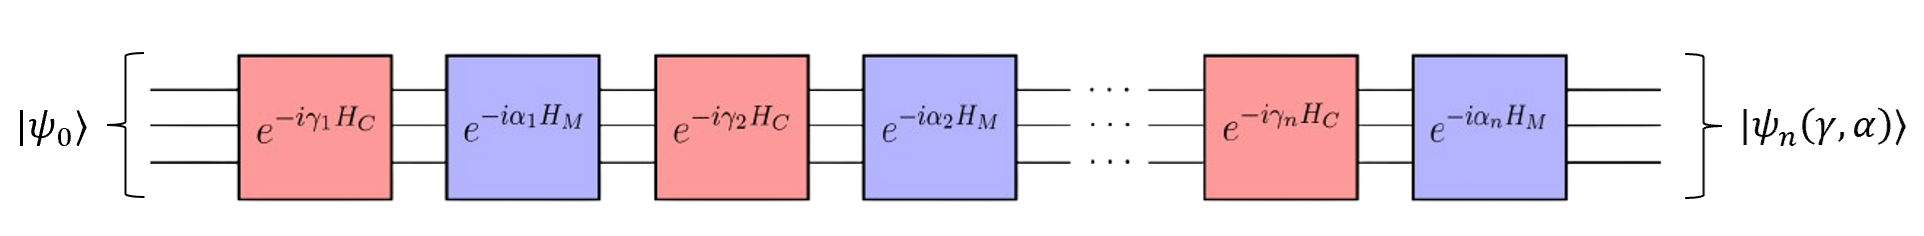
\includegraphics[width = \linewidth]{Figures/Diagrams/QAOA_Trotterization.png}
    \caption{Quantum alternating operator ansatz. Adapted from \cite{Intro_QAOA}.}
    \label{fig:QAOA_Trotterization}
\end{figure}
\noindent Replacing adiabatic time evolution with a \textit{Trotterized} evolution works due to the famous Trotter-Suzuki formulas \cite{nielsen2010quantum}, which state that (for general non-commuting $H_j$):
\begin{equation}
    e^{-i\sum_{j=1}^{m}H_{j}t}=\prod_{j=1}^{m}e^{-i H_{j}t}+O(m^{2}t^{2}).
\end{equation}
If $t \ll 1$, then the error in this approximation becomes negligible. On the other hand, if $t$ is large, Trotter-Suzuki formulas can still be used to simulate the dynamics accurately by breaking things up into a sequence of short time-steps. Let $r$ be the number of steps taken in the time evolution, so each time-step runs for time $t/r$. Then, we have that
\begin{equation}
    e^{-i\sum_{j=1}^{m}H_{j}t}=\left(\prod_{j=1}^{m}e^{-i H_{j}t/r}\right)^{r}+O(m^{2}t^{2}/r),
\end{equation}
which implies that if $r$ scales as $m^2t^2/\epsilon$, then the error can be made at most $\epsilon$ for any $\epsilon > 0$. In the \acrshort{qaoa} case, we simply have $H = H_C + H_M$ and we treat each of the evolution time intervals as variational parameters that are optimized classically (can be seen as $t/r \equiv \gamma_l, \alpha_l$). This means we do not use this \textit{Trotterization} approach directly, but it heavily inspires the \acrshort{qaoa} ansatz nevertheless. 

Let's now further detail the practical realization of the algorithm. Reiterating, the aim of \acrshort{maxcut} is to maximize the number of edges in a graph that are "cut" by a given partition of the vertices into two sets (cf. Figure \ref{fig:MaxCut}). One way of implementing \acrshort{qaoa} for \acrshort{maxcut} is to consider: $H_C$ as in Eq. \ref{eq:H_C}, where the sum is over all edges of the studied graph, connecting vertices $(j, k)$; and $H_M = \sum_{j=1}^{N} \boldsymbol{X_j}$, for $N$ qubits and graph nodes. In this scheme, the associated cost function, $\bra{\psi_n(\boldsymbol{\gamma}, \boldsymbol{\alpha})}H_C\ket{\psi_n(\boldsymbol{\gamma}, \boldsymbol{\alpha})}$, merely rewards cases where we have edges between nodes of different sets. Furthermore, we can, now, also write\footnotemark\vspace*{-5mm}
\begin{align}
    U_{H_{C_l}} = e^{-i\gamma_l H_C} = \prod&_{\mathrm{Edge}\;(\mathrm{j,k})}e^{-i\gamma_l(1-\boldsymbol{Z}_{j}\boldsymbol{Z}_{k})/2} \\
    U_{H_{M_l}} = e^{-i\alpha_l H_M} = \prod&_{j=1}^{n}e^{-i\alpha_l\boldsymbol{X}_{j}}
\end{align}
These give us the form of the unitaries that are applied in each layer of the \acrshort{qaoa} ansatz, representing the \textit{Trotter}-inspired time evolution of Figure \ref{fig:QAOA_Trotterization} (red and blue boxes). They correspond to the complex exponentials of the cost and mixer Hamiltonians, respectively: $e^{-i\gamma_l H_C}$ and $e^{-i\alpha_l H_M}$. Notice how $U_{H_{M_l}}$ uses Pauli-$x$ operators, instead of the usual Pauli-$z$ in $U_{H_{C_l}}$. In practice, the mixer Hamiltonian terms $e^{-i\alpha_l H_M}$ correspond to $R_x(2\alpha_l)$ and are easy to implement. The cost Hamiltonian terms, on the other hand, are a bit more tricky, requiring the use of $2$ CNOT gates. Each of the terms $e^{-i\gamma_l(1-\boldsymbol{Z}_{j}\boldsymbol{Z}_{k})/2}$ can be transpiled into a quantum circuit, as shown in Figure \ref{fig:Z_iZ_jDecomposition}, below. For each edge in the graph, we'll have one of these terms, in each of the $n$ layers of the \acrshort{qaoa} ansatz.
\begin{figure}[H]
  \centering
  \begin{quantikz}
  \lstick{Qubit $i$} & \ctrl{1} & \qw                & \ctrl{1}  & \qw & \\
  \lstick{Qubit $j$} & \targ{}  & \gate{R_z(\gamma_l)} & \targ{}   & \qw & \\
  \end{quantikz}
  \caption{$e^{i\gamma_l \boldsymbol{Z}_{i} \boldsymbol{Z}_{j} /2}$ decomposition.}\label{fig:Z_iZ_jDecomposition}
\end{figure}
\noindent This allows us to re-write Eq. \ref{eq:Psi_p} as
\begin{equation}
     \ket{\psi_n(\boldsymbol{\gamma}, \boldsymbol{\alpha})} = U_{H_{M_n}}U_{H_{C_n}} ... U_{H_{M_1}}U_{H_{C_1}}\ket{\psi_0}
\end{equation}
In \acrshort{qaoa}, it is customary to start with a uniform superposition over the $N$ bit-string basis states, where $N$ represents the number of graph nodes. This is denoted as $\ket{\psi_0} = \ket{+}^{\otimes N}=\frac{1}{\sqrt{2^{N}}}\sum_{z\in\{0,1\}^{N}}\ket{z}$, and is achieved by applying a Hadamard gate to each of the qubits, at the start of the quantum circuit.

Subsequently, a classical routine is employed to optimize the values of the parameters by minimizing the negative of the cost (analogous to the "cut"), therefore enabling the extraction of the \acrshort{maxcut} partition. Experimentally, for each step of the classical optimization, it is necessary to compute expectation values of Pauli-$z$ operators, which requires the quantum circuit to be sampled a certain number of times (shots). Additionally, in case it was not yet clear, note that in \acrshort{qaoa} we use one qubit for each node of the graph, with the qubits' values indicating which set they correspond to: $\ket{0}$: "Set 0"; $\ket{1}$: "Set 1". As such, for the graph in Figure \ref{fig:MaxCut}, we'd require $5$ qubits. Exemplifying, if the most sampled basis state at the end of the quantum circuit is $\ket{00011}$, then nodes $1$, $2$ and $3$ belong to "Set 0", while nodes $4$ and $5$ belong to "Set 1".

% I think I should include the "sample simulations" in the "Implementations" section, not here.

%%%%%%%%%%%%%%%%%%%%%%%%%%%%%%%%%%%%%%%%%%%%%%%%%%%%%%%%%%%%%%%%%%%%%%%%
\subsubsection{Variational Qubit-Efficient MaxCut Heuristic Algorithm (QEMC)}
\label{subsubsection:QEMC}

% Re-read all of this!

The Qubit-Efficient \acrshort{maxcut} Heuristic Algorithm (\acrshort{qemc}) \cite{tenecohen2023variational} is somewhat similar to \acrshort{qaoa}. After all, it was heavily inspired by it. However, it has a number of crucial differences. First, it only requires $n = \log_2(N)$ qubits, instead of $N$, where $N$ is the number of nodes in the graph. Additionally, the \acrshort{qemc} algorithm is based on a novel probability threshold encoding scheme, a suitable cost function, and a parameterized unconstrained quantum circuit. Going in order:

% Kind of a subsubsubsection.
\subsubsection*{\small Probability threshold encoding scheme}
With $n$ qubits, each of the $N = 2^{n}$ basis states will represent one of the graph's nodes. Following the sampling of the quantum circuit, a probability distribution is generated. Nodes with probabilities exceeding a certain threshold, $p_{th} = \frac{1}{2B}$, belong to "Set 1", while probabilities below this value indicate inclusion in "Set 0". This strongly diverges from how we encode set inclusion in \acrshort{qaoa}.

% Kind of a subsubsubsection.
\subsubsection*{\small Suitable cost function}
The objective function utilized in QEMC is the following:
\begin{equation}
L(\{p(i)\}) = \sum_{\stackrel{j < k:}{(j,k)\in E}}\left[\left(d(j,k)-\frac{1}{B}\right)^{2}+\left(s(j,k)-\frac{1}{B}\right)^{2}\right],
\end{equation}
where $d(j,k) = |p(j) - p(k)|$ and $s(j, k) = p(j) + p(k)$ are the absolute difference and sum of the corresponding basis states' probabilities. The idea is that as both $d(j, k)$ and $s(j, k)$ tend towards $1/B$, the probability of one node approaches zero (distinctive "Set 0"), while the probability of the other node approaches $1/B$ (distinctive "Set 1"), without specifying which is which. Ultimately, just like for \acrshort{qaoa}, connections between nodes of different sets are favoured. Note, however, that this probability threshold encoding scheme assumes \textit{a priori} that one of the sets ("Set 1") has $B$ nodes. Nevertheless, this is not an issue, as we can efficiently iterate through all potential values of $B\,=\,1,...,\left\lfloor{\frac{N}{2}}\right\rfloor$. Frequently, it is reasonable to set $B = N/2$, and we shall use this as our default starting point.

% Kind of a subsubsubsection.
\subsubsection*{\small Problem-agnostic ansatz}
The \acrshort{qemc} circuit ansatz is agnostic to specific graph instances, a departure from \acrshort{qaoa} where the graph structure is explicitly encoded in the quantum circuit. Instead, the graph is implicitly encoded through the cost function. As a result, the \acrshort{qemc} quantum circuit is not bound to any particular form and only needs to be expressive enough to approximate the optimal states in the Hilbert space. Such problem-independent ansatz approach provides considerable flexibility in ansatz selection. Frequently, the circuit ansatz known as "Strongly Entangling Layers" is employed, as depicted below (Figure \ref{fig:Strongly_Entangling_Layers}). As can be seen, this ansatz applies a series of parameterized single-qubit rotations interspersed with entangling gates to generate a highly entangled quantum state. We use PennyLane's \href{https://docs.pennylane.ai/en/stable/code/api/pennylane.StronglyEntanglingLayers.html}{\texttt{qml.StronglyEntanglingLayers}} implementation for this purpose.

\begin{figure}[H]
    \centering
    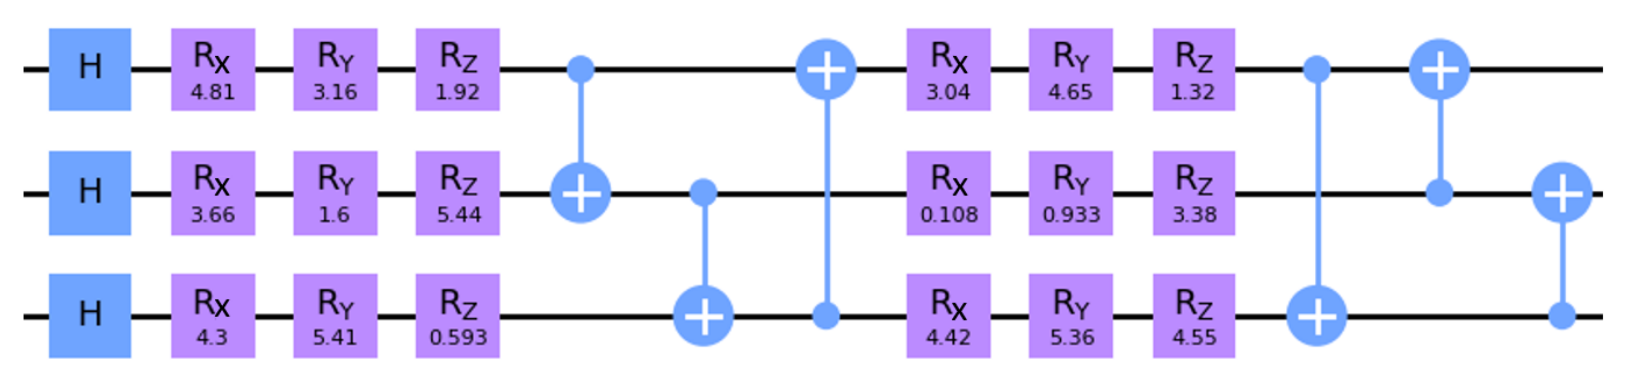
\includegraphics[width = 0.85\linewidth]{Figures/Diagrams/Strongly_Entangling_Layers.png}
    \caption{"Strongly Entangling Layers" circuit ansatz: case of $n = 3$ qubits and $p = 2$ layers. After a single layer of Hadamard gates, each subsequent layer consists of $3n$ single-qubit parameterized rotation gates and $n$ CNOT gates (entangling gates). Reproduced from \cite{tenecohen2023variational}.}
    \label{fig:Strongly_Entangling_Layers}
\end{figure}

These constitute the main ingredients necessary to understand the \acrshort{qemc} algorithm. At this point, the same hybrid loop as before would be run, so as to optimize the "Strongly Entangling Layers" ansatz's parameters, to minimize the cost function. To read the \acrshort{maxcut} partition, generated by the \acrshort{qemc} algorithm, one would sample the circuit's output one more time, after the training, and build the basis states' probability distribution. The threshold $p_{th}$ would then be applied to determine each nodes' set inclusion, from each of their associated basis states' probabilities.

One notable, and perhaps unfortunate, property of \acrshort{qemc} is that it is efficiently simulable classically. Due to the exponential compression of the number of qubits, the algorithm can be feasibly simulated on a classical computer, even for large graphs, hence defeating its purpose as a quantum algorithm. This is something the authors of the algorithm \cite{tenecohen2023variational} realized in hindsight. For this reason, it is now termed a quantum-inspired classical algorithm.

\footnotetext{In reality, \acrshort{qaoa} in this form doesn't require the use of \textit{Trotterization}, since all the operators in the sums constituting $H_C$ and $H_M$ commute. Nevertheless, it is \textit{Trotter}-inspired.}

% I'm missing the "Implementation" part, here. Also, re-read all of this!

% Include/remove "Review"?

% Describe QEMC - Explain how it works, its advantages and disadvantages, and its potential applications.

% The reason why we can efficiently iterate through the values of $B$ is that we have a reduced number of qubits (exponential compression). [I think so, at least.] We always say the set with $B$ blue nodes is the smallest. Aka., $B \leq N/2$, where $N$ is the graph's number of nodes.

% Is there any reason for this, though? What would happen if we said $B > N/2$? (Aka., the blue set is the one with the most nodes.)

% Mention that the problem-agnostic "Strongly-Entangling-Layers" ansatz might result in "too much entanglement", thus hindering the results.

% Go over the last paragraph of the QEMC section again. Something about the discussion on "shot number" is bugging me.